%!TEX root = wine_cellar.tex
\documentclass[conference]{IEEEtran}
\IEEEoverridecommandlockouts
% The preceding line is only needed to identify funding in the first footnote. If that is unneeded, please comment it out.
\usepackage{cite}
\usepackage{url}
\usepackage{tikz}
\usetikzlibrary{positioning,arrows.meta}
\usepackage{pgfplots}
\pgfplotsset{compat=1.17}
\usepackage{amsmath,amssymb,amsfonts}
\usepackage{algorithmic}
\usepackage{graphicx}
\usepackage{textcomp}
\usepackage{xcolor}
\usepackage{enumitem}
\usepackage{tabularx}
\newcolumntype{Y}{>{\raggedright\arraybackslash}X}
% DRAFT: red notes mark open questions for the team. Remove before submission.
\newcommand{\todo}[1]{\textcolor{red}{[TODO: #1]}}
\def\BibTeX{{\rm B\kern-.05em{\sc i\kern-.025em b}\kern-.08em
    T\kern-.1667em\lower.7ex\hbox{E}\kern-.125emX}}
% technology logo with a figure caption under it, kept together in one box: \logofig{python}{Python}
\newcommand{\logofig}[2]{\par\medskip\noindent\begin{minipage}{\linewidth}\centering\includegraphics[height=2.6em,width=7em,keepaspectratio]{images/logos/#1.png}\par\vspace{3pt}\refstepcounter{figure}{\footnotesize Fig.~\thefigure.~#2}\end{minipage}\par\medskip\noindent\ignorespaces}
% screenshot with a sub-label under it: \shot[width as fraction of the column]{file}{label}
\newcommand{\shot}[3][0.48]{\begin{minipage}[t]{#1\columnwidth}\centering\includegraphics[width=\linewidth]{images/screens/#2}\par\vspace{1pt}{\footnotesize #3}\end{minipage}}
\begin{document}

\title{OmniCave: Wine Cellar Management with AI Critics, designed for Transparent Display Doors
}

\author{
\makebox[\textwidth][c]{%
\begin{minipage}[t]{0.245\textwidth}
\centering
\textbf{Naomi K. Fossaberg}\\
\textit{Department of}\
\textit{Computer Science}\\
IT University of Copenhagen\\
Copenhagen, Denmark\\
{\footnotesize nafo@itu.dk}
\end{minipage}%
\hfill
\begin{minipage}[t]{0.245\textwidth}
\centering
\textbf{Enkhbold Myagmarjav}\\
\textit{Department of}\
\textit{Information Systems}\\
Hanyang University\\
Seoul, Republic of Korea\\
{\footnotesize enkheeboldu@hanyang.ac.kr}
\end{minipage}%
\hfill
\begin{minipage}[t]{0.245\textwidth}
\centering
\textbf{Chiang Jun Han}\\
\textit{Department of Electrical}\
\textit{and Electronic Engineering}\\
Nanyang Technological\\
University\\
Singapore\\
{\footnotesize jchiang009@e.ntu.edu.sg}
\end{minipage}%
\hfill
\begin{minipage}[t]{0.245\textwidth}
\centering
\textbf{Sungbin Bae}\\
\textit{Department of}\
\textit{Mathematics}\\
Hanyang University\\
Seoul, Republic of Korea\\
{\footnotesize charliepro@hanyang.ac.kr}
\end{minipage}%
}
}

\maketitle
\raggedbottom
\begin{abstract}
The premium home appliance sector increasingly competes on artificial intelligence (AI) and user experience (UX) rather than hardware specifications. Yet commercial wine cellars remain passive climate-control units, and third-party cellar apps require manual tracking with no link between the physical racks and the digital record. This paper presents OmniCave, a cloud-powered wine cellar management system designed for transparent display doors. Each bottle's label is read once when it is stored, using Amazon Rekognition and a catalog match; the system suggests a free position, tracks every bottle in centimeter coordinates, and reconciles successive cellar scans into inventory changes, including freely stacked bottles. Four fictional AI critics, each a Low-Rank Adaptation (LoRA) adapter on a shared Qwen2.5-7B model served by vLLM, debate any bottle using retrieved evidence. On unseen wines, 98--100\% of the adapters' answers pass every check (the critic's own scoring scale, the expected length, and facts taken only from the evidence), against 0--28\% for the base model with the same prompt and evidence. The door display, an Android app, and an iOS app share one cloud backend and stay synchronized over WebSocket, so the appliance runs as a thin client within the cellar's thermal and memory limits.
\end{abstract}

\begin{IEEEkeywords}
Smart Home Appliance, Cloud Computing, Vision AI, Large Language Model (LLM), Low-Rank Adaptation (LoRA), Wine Management System, Human-Computer Interaction (HCI)
\end{IEEEkeywords}

\par\smallskip
\noindent\begin{minipage}{\columnwidth}
\centering
\refstepcounter{table}\label{tab:role-assignments}
{\footnotesize TABLE \Roman{table}. \textit{Role Assignments}\par}
\smallskip
\footnotesize
\setlength{\tabcolsep}{3pt}
\renewcommand{\arraystretch}{1.05}
\begin{tabularx}{\columnwidth}{|>{\raggedright\arraybackslash}p{0.24\columnwidth}|>{\raggedright\arraybackslash}p{0.19\columnwidth}|Y|}
\hline
\multicolumn{1}{|c|}{Roles} & \multicolumn{1}{c|}{Name} & \multicolumn{1}{c|}{Task Description} \\
\hline User & Chiang Jun Han & Describe typical user scenarios and workflows. Identify usability problems and practical needs. Try prototypes and provide feedback. \\
\hline Customer & Naomi K. Fossaberg & Define the project's purpose and desired outcomes. Prioritize requirements and features. Evaluate whether the final solution meets the agreed requirements. \\
\hline Software developer & Enkhbold Myagmarjav & Design and implement software components. Write and review code. Test functionality and fix bugs. \\
\hline Development manager & Sungbin Bae & Plan tasks, milestones, and deadlines. Coordinate collaboration and monitor progress. Identify risks and help resolve blockers. \\
\hline
\end{tabularx}
\end{minipage}\par\smallskip

\section{Introduction}

\subsection{Motivation}
In recent years, the premium home appliance market has undergone a fundamental paradigm shift, transitioning from pure hardware performance competition toward elevating user experience (UX) through Cloud-based Artificial Intelligence (AI) and the seamless connectivity of the Internet of Things (IoT). High-end luxury product lines, such as LG SIGNATURE~\cite{lgsignature}, incur substantial hardware manufacturing costs, thereby demanding sophisticated, cloud-backed software capabilities that deliver commensurate value to justify their premium positioning. Concurrently, the global expansion of the fine wine market has driven rapid demand for specialized home wine cellars driven by AI management. However, existing commercial wine cellars remain passive, isolated appliances limited to fundamental condition control (temperature, humidity regulation, anti-vibration, and so on), failing to leverage vast cloud computing resources to satisfy the sophisticated digital management needs of modern fine wine collectors.

\subsection{Problem Statement and Target Audience}
The primary target demographic for luxury wine cellars consists of high-net-worth individuals, predominantly in their 40s to 60s. Although these collectors frequently possess extensive and valuable wine collections, current management paradigms introduce critical usability bottlenecks:
\begin{enumerate}
    \item \textbf{High Interaction Cost and Friction:} Existing mobile-app-based wine management solutions force users to repeatedly handle cold bottles while operating small smartphone screens. This physical separation between the appliance and the management interface induces high cognitive load and interaction friction.
    \item \textbf{Absence of Physical-Digital Synchronization:} Current wine cellars lack real-time synchronization between physical storage and digital databases. Consequently, users are required to perform manual inputs for every bottle movement, leading to severe tracking discrepancies and user abandonment over time.
\end{enumerate}

\subsection{Related Software and Limitations}
An analysis of existing wine management software (e.g., Vivino~\cite{vivino}, CellarTracker~\cite{cellartracker}) and proprietary cellar tracking apps reveals distinct functional limitations when applied to high-end collections:
\begin{itemize}
    \item \textbf{Absence of Spatial Awareness:} Most commercial applications function merely as flat digital ledgers or list-based inventories. They lack a robust spatial mapping mechanism that correlates a specific bottle's data with its exact physical coordinates (e.g., specific racks and rows) within the cellar, inevitably forcing users to manually search through shelves.
    \item \textbf{Static Data without Environmental Context:} Existing software operates completely independently of the cellar's internal hardware sensors. Consequently, they cannot factor real-time environmental data---such as multi-zone temperature differences---into their aging algorithms or serving readiness calculations.
    \item \textbf{Reactive and Monotone User Experience:} Current tools are inherently reactive, requiring users to explicitly query the database to check a wine's optimal drinking window or food pairing suitability. Furthermore, they rely on static text reviews, lacking the proactive intelligence and dynamic, expert-level engagement necessary to autonomously curate an immersive experience.
\end{itemize}

\subsection{Proposed Solution and Key Contributions}
To overcome these limitations, this paper proposes a cloud-powered, AI-driven wine cellar management system integrated with a transparent display door. Designed specifically for luxury appliances such as the LG SIGNATURE line, the proposed architecture leverages the robust computing infrastructure of centralized datacenters (e.g., LG Datacenter) to deliver uncompromising performance.

The key contributions of this work are summarized as follows:
\begin{itemize}
    \item \textbf{Label Recognition and Centimeter-Level Spatial Mapping:} Reads each bottle's label and vintage once, when the bottle is stored (Amazon Rekognition text detection matched against a wine catalog), suggests a free position, and asks the owner to confirm. Bottles are tracked in centimeter coordinates rather than rigid slots, including bottles stacked on top of one another, and a reconciliation engine turns successive cellar scans into new, moved, removed, and hidden bottles.
    \item \textbf{Cloud-Backed Multi-Agent LLM Architecture:} Replaces resource-constrained edge computing with a high-performance cloud backend (LG Datacenter). This paradigm shift allows the system to deploy massive, state-of-the-art Large Language Models (LLMs) without imposing any thermal, processing, or memory constraints on the cellar appliance itself. The cloud architecture orchestrates multi-agent dialogues among four critics, each a LoRA adapter trained on verified, evidence-grounded data: on unseen wines the adapters keep their critic's scoring scale and grounded facts in 98--100\% of answers, against 0--28\% for prompting alone, at a training cost of under five dollars.
    \item \textbf{AI-Driven UX Enhancement:} Transcending basic touch interactions, the cloud-integrated AI engine drastically elevates the overall user experience. By analyzing multidimensional real-time data, the system proactively offers a broad spectrum of personalized management features---such as optimal drinking window alerts and dynamic food pairings---transforming passive wine storage into an actively managed ecosystem.
    \item \textbf{Multi-Device Distributed Scalability:} Establishes a synchronized system architecture that seamlessly unifies multiple physical cellar units under a single user profile. Leveraging cloud centralization, it guarantees real-time synchronization between the mobile application and the appliance, eradicating tracking discrepancies.
\end{itemize}

\section{Requirements}

\subsection{Functional Requirements}

\subsubsection{User Management}
\begin{itemize}
    \item The system shall allow a user to create an account with the following mandatory information: username, email, password, and birth date, together with consent to the required terms and privacy policies. Only adults (19 or older under the Korean Youth Protection Act) may register.
    \item The system shall allow a registered user to log in with a username or email and to log out.
    \item The system shall verify a user's email address with a one-time code and allow a forgotten password to be reset by email.
    \item The system shall allow an authenticated user to edit their profile information.
\end{itemize}

\subsubsection{Inventory Mapping}
\begin{itemize}
    \item The system shall automatically detect wine bottles placed inside the wine cellar using computer vision.
    \item The system shall extract wine label information from detected bottles using AI.
    \item The system shall automatically register newly detected bottles in the inventory.
    \item The system shall automatically associate each detected bottle with a physical location in the wine cellar.
    \item The system shall automatically update a bottle's location when it is moved within the wine cellar.
    \item The system shall assign a unique identifier to each physical wine bottle to prevent duplicate inventory records.
    \item The system shall allow an authenticated user to review and correct AI-extracted wine information before confirming registration.
    \item The system shall automatically detect stacked wine bottles.
    \item The system shall automatically remove a bottle from the inventory when it is removed from the wine cellar.
    \item The system shall allow an authenticated user to manually add a wine bottle to the inventory.
    \item The system shall allow an authenticated user to manually modify bottle information.
    \item The system shall allow an authenticated user to manually remove a wine bottle from the inventory.
\end{itemize}
These requirements describe the target appliance. The prototype implements label recognition, registration, location mapping, and scan reconciliation in full; the in-cellar scans themselves come from a simulator because no cellar hardware was available (Section~\ref{sec:limitations}).

\subsubsection{Inventory Search \& Visualization}
\begin{itemize}
    \item The system shall allow a user to search for a bottle by wine name, winery, region, vintage or grape variety.
    \item The system shall display the physical location of a selected bottle within the wine cellar.
    \item The system shall display a visual map of bottles stored in the wine cellar.
\end{itemize}

\subsubsection{Environmental Monitoring}
\begin{itemize}
    \item The system shall collect environmental data from the wine cellar sensors.
    \item The system shall store historic environmental measurements from the wine cellar.
    \item The system shall associate environmental conditions with individual bottle locations.
    \item The system shall notify users when temperature or humidity exceeds user-defined thresholds for a specified duration.
    \item The system shall notify users when sensors become disconnected or environmental data is outdated.
\end{itemize}

\subsubsection{AI Recommendations}
\begin{itemize}
    \item The system shall allow a user to input data regarding a meal and receive wine pairing recommendations from the user's current inventory.
    \item The system shall allow a user to select a specific wine from the inventory and generate complementary food pairing suggestions, including culinary recipes or food delivery menu categories.
    \item The system shall recommend bottles that have reached their optimal drinking window.
    \item The system shall notify a user when wines are approaching their optimal drinking window.
    \item The system shall generate personalized recommendations based on historical consumption patterns.
    \item The system shall allow a user to input specific constraints, such as a target budget, flavor profile, or event theme, to request a curated wine list.
    \item The system shall automatically generate and display a customized wine list that satisfies the user-defined parameters, utilizing both the existing cellar inventory and a reference wine catalog for potential new purchases.
    \item The system shall recommend suitable storage locations for newly added bottles.
    \item The system shall recommend wines via natural language queries processed by the cloud-based LLM.
\end{itemize}

\subsubsection{Personalized Daily Wine Briefing}
\begin{itemize}
    \item The system shall aggregate daily wine news from external RSS feeds (e.g., Decanter and VinePair).
    \item The system shall personalize the aggregated news content by cross-referencing it with the user's specific cellar inventory, highlighting articles relevant to their owned regions, grapes, or producers.
    \item The system shall automatically curate and display a ``Daily Wine Briefing'' on the cellar's front display, including inventory-specific insights (e.g., wines reaching their peak, humidity stability).
\end{itemize}

\subsubsection{Market Value Integration}
\begin{itemize}
    \item The system shall integrate with external wine market APIs (WineAPI.io in the prototype) to retrieve current pricing data, where available, for the wines stored in the cellar, and fall back to a clearly labelled estimate otherwise.
    \item The system shall calculate and visualize the aggregated market value of the user's entire wine collection on the front display.
    \item The system shall provide graphical visualizations of estimated price trends and value appreciation for individual bottles to assist the user in asset management.
\end{itemize}

\subsubsection{Multi-Cellar Management}
\begin{itemize}
    \item The system shall allow a user to manage multiple wine cellar units and wine cellars under a single account.
    \item The system shall synchronize inventory information across connected wine cellars.
    \item The system shall allow a user to search across all connected wine cellars.
\end{itemize}

\subsubsection{Cloud-Powered Multi-Agent LLM Dialogue System}
\begin{itemize}
    \item The system shall integrate a cloud-hosted Multi-Agent Large Language Model (LLM) framework, configured with multiple distinct fictional critics, each reflecting a different scoring philosophy (e.g., a 100-point power critic, a fruit-quality purist, a value critic, and a crowd-taste critic). Real critics are not impersonated.
    \item The system shall automatically send an API request to the cloud backend to trigger a simulated multi-agent dialogue whenever a new wine is registered to the cellar inventory or actively selected by the user via the touch display.
    \item The system shall retrieve and visualize interactive, chat-style debates on the front display in real-time, showcasing diverse analytical perspectives, tasting notes, and aging predictions for the selected wine.
    \item The system shall personalize the critics' conversations and recommendations by adding a summary of the user's synchronized cellar data (inventory, consumption history, and saved preferences) to each request.
    \item \textbf{Cloud Base Model Operation:} The system shall utilize a centralized Large Language Model (LLM) hosted on a cloud GPU server as the foundational reasoning engine, run at full 16-bit precision rather than aggressively quantized for an appliance.
    \item \textbf{Server-Side Dynamic LoRA Swapping:} The system shall dynamically load and unload specific Low-Rank Adaptation (LoRA) weight matrices corresponding to the active critic on the cloud server during multi-agent dialogue generation, so that one base model in GPU memory serves every critic, each keeping its own style and scoring scale.
    \item \textbf{Continuous Critic Expansion:} The system shall allow new critics to be added through server-side LoRA adapters, and users to create their own critics described by a prompt, requiring no local software patches or model downloads on the cellar appliance.
\end{itemize}

\subsubsection{Mobile Application Integration}
\begin{itemize}
    \item The system shall provide a companion mobile application that synchronizes real-time inventory and cellar status with the user's account.
    \item The system shall allow a user to remotely browse their wine inventory, search for bottles, and view AI recommendations via the mobile application.
    \item The system shall show in-app notifications in the mobile application for critical environmental alerts (e.g., temperature fluctuations) and optimal drinking windows, delivered live over the open connection.
    \item The system shall allow a user to remotely adjust the temperature and humidity settings of individual cellar zones through the mobile application.
    \item The system shall allow a user to manually add, edit, or remove wine inventory data via the mobile application when away from the physical cellar.
\end{itemize}

\subsection{Non-Functional Requirements}

\subsubsection{Performance}
\begin{itemize}
    \item The system shall return inventory search results within 2 seconds for 95\% of requests (design target).
    \item The system shall update the displayed inventory within 10 seconds after a bottle has been added or removed (design target).
    \item The system shall process API requests to the cloud-based LLM and generate the initial multi-agent dialogue response within 1.5 seconds, utilizing token streaming to ensure a seamless user experience despite network latency.
\end{itemize}

\subsubsection{Resource \& Hardware Constraints}
\begin{itemize}
    \item The cellar's internal computing module shall function strictly as a thin client, aiming to keep local memory usage (RAM) under 1 GB by offloading all intensive Vision AI and LLM inference to the cloud.
    \item The local computing processes shall be low-power, so that their heat does not interfere with the cellar's climate control (design goal).
\end{itemize}

\subsubsection{Reliability \& Availability}
\begin{itemize}
    \item The system shall preserve the submitted data locally so that it remains after a temporary application restart.
    \item The system shall implement an offline fallback mechanism, retaining basic inventory viewing and temperature control capabilities when the Wi-Fi connection to the cloud is temporarily lost.
    \item The system shall automatically back up all inventory and configuration data to the cloud servers and support seamless recovery following an unexpected shutdown or hardware replacement.
\end{itemize}

\subsubsection{Security \& Privacy}
\begin{itemize}
    \item The system shall require secure authentication (opaque bearer tokens issued at login~\cite{bearer}) before a user can access inventory management functions across devices.
    \item The system shall securely hash and store user passwords on the cloud backend.
    \item The system shall encrypt all data transmissions between the cellar appliance, the mobile applications, and the cloud backend with HTTPS (TLS), ensuring personal consumption data and AI interactions cannot be intercepted.
    \item The system shall strictly isolate user databases on the cloud server to prevent cross-account data leaks.
    \item The system shall comply with the Korean Personal Information Protection Act (PIPA), recording separate consents (including consent to overseas transfer, since the server is in Australia) and letting users export or permanently delete their data from the cloud.
\end{itemize}

\subsubsection{Maintainability}
\begin{itemize}
    \item The system architecture shall support the server-side replacement, scaling, or upgrading of the backend LLMs without requiring firmware updates or modifications to the user interface on the cellar appliance.
    \item The system architecture shall cleanly separate the frontend UI components from the backend API services to allow independent development and deployment cycles.
\end{itemize}

\subsubsection{Usability}
\begin{itemize}
    \item The system shall provide an intuitive interface allowing new users to navigate core features without consulting external documentation.
    \item The system shall clearly indicate the current network connection status and authentication state on the main display.
    \item The system shall preserve unsaved user input locally during sudden network drops, preventing data loss before synchronizing with the cloud.
\end{itemize}

\section{Development Environment}

\subsection{Choice of Software Development Platform}

\subsubsection{Development Operating Systems}
\begin{enumerate}
    \item \textbf{Windows 11 with WSL2 (Ubuntu 22.04.5 LTS)}
\logofig{windows}{Windows 11 with WSL2} Windows 11 is selected as the primary development operating system for the backend and the integrated display because it runs all of the main project tools, including Visual Studio Code, Android Studio, Docker, and Git. Windows Subsystem for Linux 2 (WSL2) provides a full Ubuntu environment alongside Windows without a separate virtual machine, and is used for Python development, dependency management, and Docker-based workflows. Because the AWS EC2 server also runs Ubuntu, developing in WSL2 reduces differences between local and cloud environments.
    \item \textbf{macOS Tahoe 26.6.1}
\logofig{apple}{macOS Tahoe 26.6.1} macOS is selected for the native iOS application because Apple's development tools, including Xcode, the Swift compiler, SwiftUI, and the iOS Simulator, are only available on macOS. Building and testing an iOS application therefore requires at least one macOS machine within the team. Its Unix-based architecture also provides a terminal environment similar to Linux, allowing the same command-line tools and Git workflow used for the other components to be applied without modification.
\end{enumerate}

\subsubsection{Target Operating Systems}
\begin{enumerate}
    \item \textbf{Android (Android 13)}
\logofig{android}{Android} Android is selected as one of the target platforms for the companion mobile application, which gives users remote access to the system when they are away from the appliance. As the platform with the largest global smartphone market share, it is essential for reaching most potential users. The application allows users to sign in, browse and manage their inventory, monitor temperature and humidity, receive notifications, and view AI recommendations and daily news. It is developed natively with Kotlin and Jetpack Compose and stores all data through the shared FastAPI backend.
    \item \textbf{iOS (iOS 17)}
\logofig{ios}{iOS} iOS is selected as the second target mobile platform to provide the same core functionality for iPhone users. The iOS application is a separate native implementation written in Swift and SwiftUI, allowing it to follow Apple's interface guidelines rather than imitating the Android design. Although the two applications are implemented independently, both use the same FastAPI backend and API contracts. As a result, business logic and data remain centralized, and an inventory change made on one device is reflected consistently on all other clients.
    \item \textbf{webOS Open Source Edition (2.28.0)}
\logofig{webos}{webOS Open Source Edition} webOS Open Source Edition (OSE)~\cite{webos} is selected as the primary target operating system for the transparent display to ensure seamless integration with LG Electronics' commercial ecosystem, as webOS serves as the native OS for LG's premium smart home appliances, including the target LG SIGNATURE line. Technically, because webOS natively supports applications built with standard web technologies, the frontend is implemented as a React and TypeScript web application. This allows the interface to be developed, demonstrated in a standard browser, and hosted on Vercel during the initial phases without requiring the physical wine cellar hardware. Furthermore, by restricting communication between the thin-client display and the cloud-based LLM strictly to APIs, the frontend can be seamlessly ported to commercial webOS appliances without requiring any modifications to the backend services.
\end{enumerate}

\subsubsection{Programming Languages}
\begin{enumerate}
    \item \textbf{Python (3.12)}
\logofig{python}{Python} Python is selected as the primary backend language because of its readable syntax and extensive libraries for web services, data processing, computer vision, and artificial intelligence. It implements the FastAPI backend, inventory and cellar management logic, environmental sensor data processing, bottle localization, and requests to external LLM services. Using one language for both application services and data processing reduces the complexity of integrating image recognition and AI-powered recommendations into the backend. The backend runs in a Python 3.12 Docker container on AWS EC2, so all developers and the server use the same interpreter version.
    \item \textbf{TypeScript (5.9.3)}
\logofig{typescript}{TypeScript} TypeScript is selected for the integrated display because it extends JavaScript with static typing that detects many errors during development rather than at runtime. The display processes structured data from the backend, including wine metadata, bottle identifiers, storage positions, sensor readings, and AI responses. Defining these structures as TypeScript interfaces that mirror the API responses allows integration errors to be caught at compile time. TypeScript is used with React to implement the visual cellar map, inventory search, bottle details, and AI conversation interface.
    \item \textbf{Kotlin (2.2.10)}
\logofig{kotlin}{Kotlin} Kotlin is selected for the native Android application because it is Google's recommended language for Android development and integrates directly with Android Studio, the Android SDK, and Jetpack Compose. Its concise syntax reduces boilerplate code compared to Java, and its null-safety system prevents runtime errors caused by missing values in backend responses. Kotlin coroutines allow network requests to run without blocking the user interface. It is used to implement authentication, navigation, inventory management, environmental monitoring, and communication with the backend.
    \item \textbf{Swift (6.4)}
\logofig{swift}{Swift} Swift is selected for the native iOS application because it is Apple's primary programming language and integrates directly with SwiftUI and the iOS SDK. Its strong type system and optional types make the handling of missing or invalid data explicit, reducing errors when decoding backend responses. Its async/await concurrency model allows network requests to be written clearly without blocking the user interface. Swift is used to implement navigation, authentication, inventory operations, environmental monitoring, and AI-related interactions with the FastAPI backend.
    \item \textbf{SQL (PostgreSQL Dialect)}
\logofig{postgresql}{SQL} SQL is selected for managing the relational data at the core of the system. The database maintains relationships between users, wine products, individual physical bottles, cellar units, storage positions, and environmental measurements; many bottles can refer to the same wine product while each keeps its own identifier and location. Primary keys, foreign keys, and constraints enforce these relationships and prevent inconsistent records. Queries are written directly in SQL through a thin database layer that runs the same statements on PostgreSQL in production and on SQLite during local development, so no ORM is needed.
\end{enumerate}

\subsubsection{Cloud Infrastructure}
\begin{enumerate}
    \item \textbf{Amazon Web Services (AWS) -- Amazon EC2}
\logofig{ec2}{Amazon EC2} While the commercial deployment of the system is designed to leverage the enterprise-grade infrastructure of LG Datacenter for security and ecosystem integration, Amazon Web Services (AWS) EC2~\cite{aws} is selected as the cloud hosting environment for the development and prototyping phase. EC2 provides configurable virtual machines that effectively simulate a corporate datacenter environment with full control over the operating system, networking, and deployed software. A single Linux t3.small instance runs the FastAPI backend and the Caddy web server~\cite{caddy} (automatic HTTPS) in Docker containers coordinated by Docker Compose, while the database runs on Amazon RDS for PostgreSQL 17. Mirroring the target architecture---where heavy LLM inference is offloaded to dedicated GPU clusters within the LG Datacenter---the prototype delegates language model processing to a separate GPU server (RunPod, below). Consequently, no GPU is required on this instance, and the 2 vCPU and 2 GB RAM configuration is sufficient for the core backend logic. This architecture successfully provides one central backend that seamlessly synchronizes the integrated thin-client display and the companion mobile applications.
    \item \textbf{Amazon RDS for PostgreSQL}
\logofig{rds}{Amazon RDS} The database runs on a managed Amazon RDS instance (PostgreSQL 17, db.t4g.micro) rather than on the EC2 server. RDS handles storage, minor-version patching, and automated daily backups (kept for seven days), and the instance is not publicly accessible: only the EC2 server inside the same virtual private cloud can connect to it. Because the EC2 server keeps no data of its own, it can be rebuilt or replaced at any time without data loss.
    \item \textbf{Amazon Rekognition}
\logofig{rekognition}{Amazon Rekognition} Amazon Rekognition's text detection (DetectText) reads the text on a wine label photographed with the mobile app. The backend sends the photo with the AWS SDK, using the EC2 instance's IAM role instead of stored access keys, and matches the detected words against its wine catalog. Using a managed service keeps image analysis in the cloud, in line with the thin-client design, and requires no model hosting.
    \item \textbf{WineAPI.io:} Market prices come from the WineAPI.io REST API (public beta). To stay within the free plan of 100 requests per day, the backend refreshes each wine at most once a day in the background and caches the result in the database.
    \item \textbf{Vercel}
\logofig{vercel}{Vercel} Vercel is selected to host the React-based integrated display because it specializes in deploying frontend web applications and supports Vite projects without additional configuration. Its GitHub integration automatically builds and deploys the application when changes are pushed, and creates preview deployments for branches so that interface changes can be reviewed before merging. The deployed display retrieves inventory, cellar status, environmental readings, and AI results from the FastAPI backend. Hosting the frontend separately allows it to be developed and deployed independently of the backend.
    \item \textbf{RunPod GPU Cloud and vLLM (Critic Model Serving)}
\logofig{runpod}{RunPod} While the commercial system is intended to run inside the LG Datacenter, the prototype rents a GPU on RunPod only when needed (training and demo sessions). The open-weight Qwen2.5-7B-Instruct model is served by vLLM~\cite{vllm} together with four LoRA adapters~\cite{lora}, one per critic; vLLM selects the adapter per request, which implements server-side LoRA swapping without reloading the base model. A small gateway in front of vLLM adds the retrieved evidence for the wine (scores, prices, drinking windows, crowd ranks) to each prompt. The adapters were trained on the same platform in about two hours on one A100 GPU. Token streaming gives a first token in about 1 second through the RunPod proxy.
    \item \textbf{Mock Provider (Development and Fallback):} During development, and whenever the GPU server is off, the backend answers with a built-in mock provider so that every client remains usable without any paid service.
    \item \textbf{Architectural Decoupling:} All LLM providers (the mock provider and vLLM) are accessed through one backend interface selected by a configuration value. Moving from the prototype to a commercial LG Datacenter LLM therefore requires only a configuration change, not a refactoring of the backend logic.
\end{enumerate}

\subsubsection{Development Tools}
\begin{enumerate}
    \item \textbf{Visual Studio Code (1.144.1)}
\logofig{vscode}{Visual Studio Code} Visual Studio Code is selected as the primary code editor because it is lightweight, free, and supports Python, TypeScript, Docker, and Git through an extensive ecosystem of extensions. It provides code completion, linting, and an integrated debugger for both the FastAPI backend and the React display. Its WSL integration allows files inside the Ubuntu environment to be edited directly, and its integrated terminal allows developers to run backend services and execute Docker and Git commands without leaving the editor.
    \item \textbf{Xcode (27.2)}
\logofig{xcode}{Xcode} Xcode is selected as the development environment for the native iOS application because it is Apple's official IDE and includes the iOS SDK, the Swift compiler, and debugging and profiling tools. SwiftUI previews allow interface components to be inspected while they are being written. The iOS Simulator is used to test the application across different iPhone models and screen sizes, while testing on physical devices validates behavior and network communication outside the simulated environment.
    \item \textbf{Android Studio Rabbit 2 (2026.2.2)}
\logofig{androidstudio}{Android Studio} Android Studio is selected for the native Android application because it is Google's official IDE and provides integrated support for Kotlin, Jetpack Compose, Gradle, and the Android SDK. Compose previews allow screens to be inspected without launching the full application, and built-in profiling tools help identify performance issues. The Android Emulator is used to test the application across different device configurations and Android versions, while physical-device testing verifies behavior under practical network and hardware conditions.
    \item \textbf{Docker Engine (29.9.2) and Docker Compose (5.7.0)}
\logofig{docker}{Docker} Docker is selected to package the backend services and their dependencies into containers, ensuring that the same configuration runs on every developer's machine and on the AWS EC2 server. The FastAPI backend and the Caddy web server run in separate containers, so each can be updated or restarted independently. Docker Compose defines both containers, their internal network, environment variables, and persistent storage volumes in a single file. Any team member can start the complete backend locally with one command, and the same configuration is used for deployment.
    \item \textbf{Git (2.34.1) and GitHub}
\logofig{github}{Git and GitHub} Git is selected as the version control system because several components are developed in parallel while sharing one source code history. Each feature is developed on a separate branch and integrated through merging, while the commit history allows previous versions to be restored when necessary. GitHub hosts the central repository and adds pull requests, code reviews, and issue tracking. The repository contains separate directories for the backend, integrated display, Android application, iOS application, and documentation, and its Vercel integration automatically deploys the integrated display.
    \item \textbf{Jira}
\logofig{jira}{Jira} Jira is selected for project planning and task tracking because it provides a shared workspace for organizing development activities. The team used it to maintain the backlog, divide requirements into tasks, assign responsibilities, set priorities, and track bugs, with boards showing the progress of the backend, integrated display, mobile application, and AI integration tasks.
    \item \textbf{Draw.io (diagrams.net)}
\logofig{drawio}{Draw.io} Draw.io is selected to create technical diagrams because it is free, runs in the browser, and stores diagrams in a format that can be tracked in the Git repository. It is used for the system architecture diagram (Fig.~\ref{fig:architecture}), whose source file is kept in the repository next to the exported image.
    \item \textbf{LaTeX}
\logofig{latex}{LaTeX} LaTeX is selected for the project documentation because it produces consistently formatted technical documents and handles tables, figures, equations, and references reliably. The team uses the IEEE conference template, as required for the course, to organize the introduction, requirements, development environment, specifications, and subsequent documentation. Because LaTeX documents are plain text, the source files are stored in the GitHub repository alongside the software, allowing documentation changes to be tracked and reviewed in the same way as source code.
\end{enumerate}

\subsubsection{AI-Assisted Development Tools}
\begin{enumerate}
    \item \textbf{Codex CLI (0.162.1; ChatGPT Plus; Astra 6.1)}
\logofig{openai}{Codex CLI} Codex CLI is a command-line coding agent developed by OpenAI, used in this project with the Astra 6.1 model through a ChatGPT Plus subscription. It works directly within the project's source files and terminal, allowing it to read existing code, propose changes, and run tests and builds. The team uses Codex mainly for implementing individual features, including backend API endpoints, React components, and database operations, as well as for debugging and writing automated tests.
    \item \textbf{Claude Code (2.1.309; Claude Pro; Opus 5.5)}
\logofig{claude}{Claude Code} Claude Code is a command-line coding agent developed by Anthropic, used in this project with the Claude Opus 5.5 model through a Claude Pro subscription. Like Codex, it works directly with the repository and development tools, but the team uses it mainly for tasks that span several components. These include refactoring code across modules, reviewing implementation approaches against the planned architecture, and checking consistency between the backend API and the data structures used by the client applications.
\end{enumerate}

\subsubsection{Computer Resources}
Table~\ref{tab:computer-resources} lists the computer resources used for development and deployment.

\par\smallskip
\noindent\begin{minipage}{\columnwidth}
\centering
\refstepcounter{table}\label{tab:computer-resources}
{\footnotesize TABLE \Roman{table}. \textit{Computer Resources}\par}
\smallskip
\footnotesize
\setlength{\tabcolsep}{3pt}
\renewcommand{\arraystretch}{1.05}
\begin{tabularx}{\columnwidth}{|>{\raggedright\arraybackslash}p{0.24\columnwidth}|Y|>{\raggedright\arraybackslash}p{0.16\columnwidth}|>{\raggedright\arraybackslash}p{0.12\columnwidth}|}
\hline
\multicolumn{1}{|c|}{Resource} & \multicolumn{1}{c|}{Device / OS} & \multicolumn{1}{c|}{CPU} & \multicolumn{1}{c|}{RAM} \\
\hline Naomi K. Fossaberg & MacBook Air 13-inch (2024), macOS Tahoe 26.6.1 & Apple M3 & 16 GB \\
\hline Enkhbold Myagmarjav & ASUS Zenbook 14 (UX3405MA), Windows 11 Home (Build 26300) & Intel Core Ultra 7 155H (16 cores, 22 threads) & 16 GB \\
\hline Chiang Jun Han & Windows 11 Home 25H2 & Intel Core i9-13900H (2.60 GHz) & 32 GB \\
\hline Sungbin Bae & Windows 11 & Intel Core i7-12700F (2.10 GHz) & 32 GB \\
\hline AWS EC2 (t3.small) & Ubuntu 24.04 LTS, 20 GB gp3 storage, Sydney region & 2 vCPU & 2 GB \\
\hline
\end{tabularx}
\end{minipage}\par\smallskip

\subsubsection{Cost Estimation}
\mbox{}\par\smallskip
\noindent\begin{minipage}{\columnwidth}
\centering
\refstepcounter{table}\label{tab:cost-estimation}
{\footnotesize TABLE \Roman{table}. \textit{Estimated Development Cost}\par}
\smallskip
\footnotesize
\setlength{\tabcolsep}{3pt}
\renewcommand{\arraystretch}{1.05}
\begin{tabularx}{\columnwidth}{|Y|>{\raggedright\arraybackslash}p{0.24\columnwidth}|}
\hline
\multicolumn{1}{|c|}{Item} & \multicolumn{1}{c|}{Cost (USD)} \\
\hline Development laptops & \$3,500 \\
\hline AWS EC2 t3.small, 20 GB storage, and public IPv4 address & \$25--30 \\
\hline Vercel (Hobby plan) & \$0 \\
\hline Amazon RDS for PostgreSQL (db.t4g.micro) & \todo{\$} \\
\hline RunPod GPU (LoRA training on A100, about 2 h) & \$4.45 \\
\hline RunPod GPU (serving for tests and demos) & \todo{\$} \\
\hline Amazon Rekognition (label text detection) & \todo{\$} \\
\hline WineAPI.io (free plan) & \$0 \\
\hline ChatGPT Plus (Codex CLI) & \$20 \\
\hline Claude Pro (Claude Code) & \$20 \\
\hline VS Code, Xcode, Android Studio, Docker, Git, GitHub, Jira, Draw.io, and LaTeX (free tools/plans) & \$0 \\
\hline \textbf{Total} & \textbf{\todo{recompute}} \\
\hline
\end{tabularx}
\end{minipage}\par\smallskip

\noindent\textbf{Cost Breakdown Notes:}
\begin{itemize}
    \item \textbf{Hardware:} Development laptops for the team, including a macOS machine required for iOS development.
    \item \textbf{Cloud Infrastructure:} An AWS EC2 t3.small instance hosts the backend and web server, including storage and a public IPv4 address, and Amazon RDS hosts the PostgreSQL database. Vercel's free Hobby plan hosts the integrated display.
    \item \textbf{AI Services:} A RunPod GPU is rented by the hour for LoRA training and for serving the critic models during tests and demonstrations.
    \item \textbf{Development Tools:} Most tools used in the project, including VS Code, Xcode, Android Studio, Docker, Git, GitHub, Jira, Draw.io, and LaTeX, are free or open source.
    \item \textbf{AI Coding Assistants:} ChatGPT Plus (Codex CLI) and Claude Pro (Claude Code) subscriptions are used throughout development.
\end{itemize}

\subsection{Software in Use}

\subsubsection{Frontend Frameworks and Build Tools}
\begin{enumerate}
    \item \textbf{React (19.3.1)}
\logofig{react}{React} React~\cite{react} is selected as the frontend library for the integrated transparent display because its component-based architecture allows the interface to be built from small, reusable elements that manage their own state. The visual cellar map, bottle information, environmental measurements, and AI conversations are each implemented as separate components. When new data is received from the backend, React updates only the affected parts of the interface without reloading the page, keeping the display responsive. Its large ecosystem and first-class TypeScript support also simplify development and maintenance.
    \item \textbf{Vite (7.3.7)}
\logofig{vite}{Vite} Vite is selected as the development server and build tool for the integrated display because it provides a fast development workflow and produces optimized assets for deployment. During development, its hot module replacement shows changes to a component in the running interface almost immediately without losing the current application state. For deployment, it bundles and minifies the application into static files served by Vercel. Using Vite keeps the frontend build process simple and independent of the backend and database infrastructure.
\end{enumerate}

\subsubsection{Backend Frameworks}
\begin{enumerate}
    \item \textbf{FastAPI (0.162.0)}
\logofig{fastapi}{FastAPI} FastAPI~\cite{fastapi} is selected as the primary backend framework because it is a modern, high-performance Python framework designed for building APIs. It uses Python type hints to validate requests and serialize responses automatically, catching malformed data before it reaches the application logic. It supports asynchronous request handling and WebSocket connections natively, and automatically generates OpenAPI documentation that serves as a shared API reference for all client applications. FastAPI implements authentication, inventory management, bottle location updates, cellar configuration, environmental monitoring, and AI service communication, so all clients share the same business logic.
\end{enumerate}

\subsubsection{Mobile Application Frameworks}
\begin{enumerate}
    \item \textbf{SwiftUI (iOS 27.2 SDK)}
\logofig{swift}{SwiftUI} SwiftUI~\cite{swiftui} is selected for the native iOS application because it is Apple's modern declarative framework for building user interfaces with Swift. Developers describe how the interface should appear for a given state, and SwiftUI updates the screen automatically when that state changes. This allows inventory, cellar, and environmental data received from the backend to be reflected immediately in the corresponding views. SwiftUI is used to build the authentication, inventory, bottle detail, environmental monitoring, and AI recommendation screens, with built-in navigation and accessibility support.
    \item \textbf{Jetpack Compose (UI/runtime 1.12.1)}
\logofig{jetpackcompose}{Jetpack Compose} Jetpack Compose~\cite{compose} is selected for the native Android application because it is Android's modern declarative UI toolkit and is fully integrated with Kotlin and Android Studio. Like SwiftUI, Compose describes the interface for a given state and automatically updates the affected components when that state changes, for example when new inventory information is retrieved from the backend. This removes the need for XML layouts and much manual view-update code. Because both mobile applications use a declarative approach, the team can follow a similar screen structure on both platforms.
\end{enumerate}

\subsubsection{Database}
\begin{enumerate}
    \item \textbf{PostgreSQL (17)}
\logofig{postgresql}{PostgreSQL} PostgreSQL~\cite{postgres} is selected as the primary database because it is a mature, open-source relational database known for its reliability and data integrity. Its transactions and relational constraints ensure that operations such as registering, moving, or removing a bottle are either fully completed or not applied at all. Indexing supports fast inventory searches by wine name, winery, region, vintage, or grape variety, while JSON data types allow semi-structured data such as AI conversation history to be stored. PostgreSQL runs on Amazon RDS with automated backups, providing one central data source for all clients.
    \item \textbf{SQLite (development)}
\logofig{sqlite}{SQLite} SQLite is used for local development and automated tests because it needs no server and stores the whole database in one file. A thin database layer issues the same SQL statements to SQLite and PostgreSQL and adapts the few differences (placeholders and returned row types), so every developer can run the full backend with one command.
\end{enumerate}

\subsubsection{Communication and Integration}
\begin{enumerate}
    \item \textbf{REST API over HTTP/HTTPS with JSON}
\logofig{json}{REST and JSON} RESTful APIs are selected as the primary communication mechanism because they provide a simple, stateless interface supported on every platform in the project. Resources such as users, wines, bottles, cellars, and sensor readings are exposed through endpoints that use standard HTTP methods (GET, POST, PUT, PATCH, and DELETE). HTTP is used during local development, while HTTPS secures the deployed backend through Transport Layer Security (TLS). Data is exchanged in JSON, which is supported in Python, TypeScript, Kotlin, and Swift, allowing all clients to use a single backend.
    \item \textbf{WebSocket:} WebSocket~\cite{websocket} is selected to support persistent, bidirectional communication for features that require continuous updates. Unlike REST requests, which require the client to ask for new data, a WebSocket connection remains open, allowing the backend to send updates to clients as soon as changes occur. It is used to transmit changes in inventory, bottle locations, environmental measurements, and cellar connection status, so that an action on one device is reflected on all other clients without repeated polling. REST APIs remain responsible for standard request-response operations.
    \item \textbf{Server-Sent Events (SSE):} AI answers (critic debates, pairings, and recommendations) are streamed from the backend to the clients as Server-Sent Events~\cite{sse}, so text appears word by word while the model is still generating.
\end{enumerate}

\subsection{Task Distribution}

\par\smallskip
\noindent\begin{minipage}{\columnwidth}
\centering
\refstepcounter{table}\label{tab:task-distribution}
{\footnotesize TABLE \Roman{table}. \textit{Task Distribution}\par}
\smallskip
\footnotesize
\setlength{\tabcolsep}{3pt}
\renewcommand{\arraystretch}{1.05}
\begin{tabularx}{\columnwidth}{|>{\raggedright\arraybackslash}p{0.24\columnwidth}|>{\raggedright\arraybackslash}p{0.19\columnwidth}|Y|}
\hline
\multicolumn{1}{|c|}{Role} & \multicolumn{1}{c|}{Name} & \multicolumn{1}{c|}{Task Description} \\
\hline iOS Application Developer & Naomi K. Fossaberg & Develop the native SwiftUI iOS application and connect it to the shared backend, including authentication, inventory, climate, critic debate streaming, notifications, and its test suite. \\
\hline Backend, Display \& Cloud Developer & Enkhbold Myagmarjav & Design and implement the FastAPI backend, the React/TypeScript door display, the native Android application, and the AWS deployment (EC2, RDS, Caddy). \\
\hline Mobile Prototype \& Testing & Chiang Jun Han & Build the first companion-app prototype; write the automated backend and Android tests and the continuous integration pipeline. \\
\hline AI Developer & Sungbin Bae & Build the critic AI: evidence retrieval, teacher-generated training data, LoRA training and evaluation on Qwen2.5-7B, and the vLLM serving gateway. \\
\hline
\end{tabularx}
\end{minipage}\par\smallskip

\section{Specifications}

\subsection{Functional Requirements}

\subsubsection{User Management}
\begin{itemize}
    \item Sign-Up
    \begin{itemize}
        \item Username Input
        \begin{itemize}
            \item Description: Users choose a public username.
            \item Input Format: 3--32 characters (letters, digits, ``\_'', ``.'', ``-'').
            \item Validation: The server rejects usernames that are already taken.
        \end{itemize}
        \item Email Input
        \begin{itemize}
            \item Description: Users enter their email with the proper format.
            \item \raggedright Input Format: [useremail]@[somemailform].[com/kr/dk/other].
            \item Validation: Check that the email input contains valid characters and verify that it follows a correct email format before allowing submission.
        \end{itemize}
        \item Password Input
        \begin{itemize}
            \item Description: Users set a password and re-enter it for confirmation.
            \item Input Format: Minimum 8 characters, requiring at least 1 lowercase letter, 1 uppercase letter, 1 number, and 1 special character.
            \item Validation: Ensure that the password meets the minimum requirements for input format.
            \item Validation: Confirm that both password inputs match. A live checklist shows which rules are met.
        \end{itemize}
        \item Birth Date Input
        \begin{itemize}
            \item Description: Users enter their birth date with a date picker.
            \item Validation: Registration is allowed from 1 January of the year the user turns 19 (Korean Youth Protection Act); only the birth year counts.
        \end{itemize}
        \item Consents
        \begin{itemize}
            \item Description: Required consents (terms of service, collection of personal information, overseas transfer) and an optional marketing consent, each with a link to the full policy and an ``Agree to all'' option.
            \item Validation: Sign-up is possible only when every required consent is given. Each consent is stored with its policy version and time.
        \end{itemize}
        \item Sign-Up Button
        \begin{itemize}
            \item Behavior: Disabled until all inputs are valid and the required consents are given.
            \item Action: Creates the account. When email verification is enabled, a 6-digit code is emailed and the account is activated after the code is entered; otherwise the user is redirected to the Log-In screen.
        \end{itemize}
    \end{itemize}

    \item Log-In
    \begin{itemize}
        \item Username or Email Input
        \begin{itemize}
            \item Description: Prompts users to enter their username or their email address.
            \item Validation: The field must not be empty.
        \end{itemize}
        \item Password Input
        \begin{itemize}
            \item Description: Prompts users to enter their password.
            \item Input Format: Password inputs are hidden and displayed as asterisks (*) to ensure privacy.
            \item Validation: Ensure that the password input meets the minimum security requirements and matches the user's registered password.
        \end{itemize}
        \item Log-In Button
        \begin{itemize}
            \item Action: Authenticates users with the provided username or email address and the password; both identifiers work.
            \item On Success: Redirects users to the Main page.
            \item On Failure: Displays the server's error message (e.g., ``Invalid username or password''). If the email is not yet verified, the user is taken to the code screen.
        \end{itemize}
    \end{itemize}

    \item Forgot Password
    \begin{itemize}
        \item Description: Lets users who forgot their password set a new one.
        \item Action: The user enters an email address and receives a 6-digit code (the answer is the same whether or not the address exists). Entering the code and a new password changes the password and ends all active sessions.
    \end{itemize}

    \item Logout
    \begin{itemize}
        \item Description: Allows authenticated users to securely end their current session.
        \item Logout Button
        \begin{itemize}
            \item Action: Clicking the ``Log Out'' button terminates the user's session, removes the active authentication token, and redirects the user to the login screen.
        \end{itemize}
    \end{itemize}

    \item Edit User Profile
    \begin{itemize}
        \item Description: Allows authenticated users to view and modify their personal account information.
        \item Feature: A profile management page displays editable fields, such as email address and password, alongside a ``Save Changes'' button.
        \item Action: After modifying their information, clicking ``Save Changes'' validates and updates the information in the database. A confirmation message is displayed when the changes are successful.
    \end{itemize}
\end{itemize}

\subsubsection{Inventory Mapping}
\begin{itemize}
    \item Automatic Wine Bottle Detection
    \begin{itemize}
        \item Description: Detects each bottle when it is placed in the cellar and keeps track of the bottles already inside.
        \item Feature: When a bottle is stored, its front label is photographed once; in the prototype the mobile app's camera stands in for an entry camera at the door. For the bottles already inside, the cellar's scans report every bottle's position in centimeters. The appliance only sends the scan; the cloud backend reconciles it with the inventory. Because no cellar hardware was available, the prototype's scans come from the edge agent's simulator through the same interface.
        \item Action: When a new bottle is detected, the system starts the identification and registration process.
    \end{itemize}

    \item Wine Label Recognition
    \begin{itemize}
        \item Description: Extracts wine information from a photo of the bottle's label using cloud image recognition.
        \item Feature: Amazon Rekognition detects the text lines on the label. The backend matches them against its wine catalog (at least 60\% of the producer and wine-name words must appear, with tolerance for misread letters) and takes the vintage from a year printed on the label; the catalog supplies the region, grape variety, and drinking window.
        \item Action: The recognized details are shown for verification before the bottle is registered. When no catalog wine matches, the review form opens with empty fields and the text that was read, so the owner can fill them in.
    \end{itemize}

    \item Automatic Bottle Registration
    \begin{itemize}
        \item Description: Automatically adds newly detected wine bottles to the user's inventory after registration is confirmed.
        \item Feature: A registration interface displays the detected wine information, the recognition confidence, and the suggested storage location.
        \item Action: After the user confirms the extracted information, the system creates a new inventory record and updates the cellar inventory.
    \end{itemize}

    \item Physical Location Mapping
    \begin{itemize}
        \item Description: Automatically associates each detected wine bottle with its physical storage location inside the cellar.
        \item Feature: Each bottle is assigned a storage coordinate in centimeters (x from the left wall, y from the floor, z from the door) together with its rack and stacking level. Racks have a nominal capacity, but bottles may be placed freely, so overfilled or irregularly packed racks are still mapped exactly.
        \item Action: For a new bottle the system suggests the best free spot (a rack in the zone suited to the wine's color, near eye level, front row first); bottles still waiting for confirmation keep their suggested spot, so two new bottles never receive the same one. When a bottle is registered, the system saves its coordinates and shows its position on the visual cellar map.
    \end{itemize}

    \item Automatic Bottle Movement Detection
    \begin{itemize}
        \item Description: Detects when an existing wine bottle is moved to a different position within the cellar.
        \item Feature: The reconciliation engine compares each scan with the stored positions; a bottle found at a new position with the same tag or a matching label is treated as moved.
        \item Action: When a previously registered bottle is detected in a new location, the system updates its corresponding storage coordinates in the inventory.
    \end{itemize}

    \item Unique Bottle Identification
    \begin{itemize}
        \item Description: Assigns a unique identifier to every physical wine bottle to prevent duplicate inventory records.
        \item Feature: Each registered bottle receives a unique bottle ID that is linked to its wine information and physical storage location.
        \item Action: When a bottle is detected again, the system checks existing inventory records to identify whether it has already been registered before creating another record.
    \end{itemize}

    \item Review and Correct Wine Information
    \begin{itemize}
        \item Description: Allows authenticated users to review and correct information extracted from wine labels before confirming registration.
        \item Feature: A wine information confirmation interface displays the AI-extracted details in editable fields.
        \item Action: Users can modify incorrect or incomplete information and select ``Confirm'' to save the corrected bottle information to the inventory.
    \end{itemize}

    \item Stacked Bottle Detection
    \begin{itemize}
        \item Description: Detects wine bottles that are stacked or partially obscured by other bottles inside the cellar.
        \item Feature: Every detection carries a three-dimensional position, so a bottle lying on top of others is identified as a separate bottle at a higher level.
        \item Action: A bottle detected above another one is registered with a stacking level and must be supported by the bottles below it; when a supporting bottle is removed, the bottles above it settle down. When identification is uncertain, the detection goes to the review queue.
    \end{itemize}

    \item Automatic Bottle Removal Detection
    \begin{itemize}
        \item Description: Detects when a registered wine bottle has been removed from the cellar.
        \item Feature: The system compares each new scan with the previously recorded bottle positions to identify missing bottles.
        \item Action: When a bottle is no longer detected, the system first checks whether it may be hidden behind another bottle. A bottle that is missing in several consecutive scans is marked as removed. Differences under 2.5 cm between scans are treated as detection noise, so positions do not drift.
    \end{itemize}

    \item Manual Bottle Registration
    \begin{itemize}
        \item Description: Allows authenticated users to manually add wine bottles that cannot be automatically detected or recognized.
        \item Feature: An ``Add Bottle'' button opens a form containing fields for wine name, winery, region, vintage, grape variety, and storage location.
        \item Action: After entering the required information and clicking ``Save'', the system generates a unique bottle ID and adds the bottle to the inventory.
    \end{itemize}

    \item Manual Bottle Modification
    \begin{itemize}
        \item Description: Allows authenticated users to modify the information associated with an existing wine bottle.
        \item Feature: Selecting a bottle opens an editable information page containing its wine details and physical storage location.
        \item Action: After modifying the information, clicking ``Save Changes'' updates the corresponding inventory record.
    \end{itemize}

    \item Manual Bottle Removal
    \begin{itemize}
        \item Description: Allows authenticated users to manually remove a wine bottle from their inventory.
        \item Feature: Each bottle's information page contains a ``Remove Bottle'' option.
        \item Action: Selecting ``Remove Bottle'' prompts the user for confirmation before removing the bottle from the active inventory.
    \end{itemize}
\end{itemize}



\subsubsection{Inventory Search \& Visualization}
\begin{itemize}
    \item Wine Inventory Search
    \begin{itemize}
        \item Description: Allows users to search for specific wine bottles stored in their cellar.
        \item Feature: A search bar and filtering options allow users to search by wine name, winery, region, vintage, or grape variety.
        \item Action: Entering a search term or selecting a filter displays all matching bottles from the inventory.
    \end{itemize}

    \item Bottle Location Display
    \begin{itemize}
        \item Description: Displays the exact physical storage location of a selected wine bottle.
        \item Feature: Each bottle's information page displays its corresponding cellar, rack, and position.
        \item Action: Selecting a bottle from the inventory highlights its physical position within the cellar.
    \end{itemize}

    \item Visual Cellar Map
    \begin{itemize}
        \item Description: Provides a graphical representation of all wine bottles stored inside the wine cellar.
        \item Feature: An interactive cellar map draws the door view to scale, with every bottle at its measured position, and a rotatable 3D view of the cellar.
        \item Action: Users can select individual bottles on the map to view their wine information and storage details.
    \end{itemize}
\end{itemize}

\subsubsection{Environmental Monitoring}
\begin{itemize}
    \item Real-Time Environmental Data Collection
    \begin{itemize}
        \item Description: Continuously collects environmental measurements from sensors installed inside the wine cellar.
        \item Feature: Temperature and humidity sensors transmit measurements per zone through the cellar's edge agent to the cloud backend. In the prototype, which has no physical sensors, the readings come from the edge agent or from a built-in simulator.
        \item Action: Upon receiving sensor readings, the system processes and displays the latest temperature and humidity values on the dashboard.
    \end{itemize}

    \item Cellar Environment History
    \begin{itemize}
        \item Description: Stores historical environmental measurements to allow users to monitor changes in cellar conditions over time.
        \item Feature: An environmental monitoring dashboard displays historical temperature and humidity measurements through graphical charts.
        \item Action: Users can select a time period to view previous environmental readings and identify changes in storage conditions.
    \end{itemize}

    \item Bottle-Specific Environmental Conditions
    \begin{itemize}
        \item Description: Associates environmental measurements with the physical storage locations of individual wine bottles.
        \item Feature: Each cellar location is linked to the relevant environmental sensor data or monitored storage zone.
        \item Action: Selecting a bottle displays the environmental conditions recorded for its corresponding storage location.
    \end{itemize}

    \item Temperature and Humidity Alerts
    \begin{itemize}
        \item Description: Notifies users when cellar temperature or humidity exceeds their predefined limits for a specified duration.
        \item Feature: Users can configure minimum and maximum temperature and humidity thresholds through the settings interface.
        \item Action: When environmental measurements exceed the configured thresholds continuously for the specified duration, the system generates a notification to alert the user.
    \end{itemize}

    \item Sensor Disconnection Alerts
    \begin{itemize}
        \item Description: Notifies users when environmental sensors become disconnected or stop transmitting updated measurements.
        \item Feature: The system monitors the latest communication timestamp from each connected sensor.
        \item Action: When a sensor fails to transmit data within the configured timeout period, the system displays a sensor disconnection or outdated data notification.
    \end{itemize}
\end{itemize}

\subsubsection{AI Recommendations}
\begin{itemize}
    \item Meal-Based Wine Recommendations
    \begin{itemize}
        \item Description: Suggests suitable wines from the user's existing inventory based on the meal they intend to consume.
        \item Feature: A meal input field allows users to describe their meal, ingredients, or preferred cuisine. The AI recommendation interface displays suitable wine selections.
        \item Action: After submitting the meal information, the system analyzes the available inventory and generates wine pairing recommendations with explanations.
    \end{itemize}

    \item Wine-Based Food Pairing
    \begin{itemize}
        \item Description: Recommends complementary food options for a specific wine selected from the user's inventory.
        \item Feature: Selecting a wine provides suggested food pairings, culinary recipes, and relevant food delivery menu categories.
        \item Action: After selecting a wine, the system generates suitable food recommendations based on its characteristics, such as grape variety, flavor profile, and acidity.
    \end{itemize}

    \item Optimal Drinking Window Recommendations
    \begin{itemize}
        \item Description: Identifies bottles that have reached their recommended drinking window.
        \item Feature: The wine information page displays the estimated drinking window and indicates whether a bottle is ready to drink.
        \item Action: The system compares the current date with the available drinking-window information and recommends bottles that have reached their optimal drinking period.
    \end{itemize}

    \item Drinking Window Notifications
    \begin{itemize}
        \item Description: Notifies users when their stored wines are approaching their recommended drinking windows.
        \item Feature: A notification section displays wines that are approaching their estimated optimal drinking periods.
        \item Action: When a bottle reaches the configured notification period before its drinking window, the system generates an alert recommending that the user consider consuming it.
    \end{itemize}

    \item Personalized Wine Recommendations
    \begin{itemize}
        \item Description: Generates wine recommendations based on the user's historical consumption patterns and preferences.
        \item Feature: The recommendation system considers previously consumed wines and saved preferences.
        \item Action: When a user requests recommendations, the system analyzes their historical consumption data and suggests wines matching their preferences.
    \end{itemize}

    \item Customized Wine List Generation
    \begin{itemize}
        \item Description: Allows users to request a curated wine list based on specific requirements.
        \item Feature: A wine list generator provides input fields for target budget, flavor profile, occasion, or event theme.
        \item Action: After submitting the selected constraints, the system filters available wines and generates a customized wine list.
    \end{itemize}

    \item Inventory and External Wine Recommendations
    \begin{itemize}
        \item Description: Generates a wine list using both the user's existing inventory and a reference wine catalog for potential purchases.
        \item Feature: Recommendation results are divided into two categories: wines currently available in the cellar and suggested wines available for purchase.
        \item Action: The system first identifies suitable wines from the existing inventory. When additional options are required, it selects matching wines from the reference catalog that the user does not own yet and displays them alongside the existing inventory recommendations.
    \end{itemize}

    \item Recommended Storage Location
    \begin{itemize}
        \item Description: Suggests suitable physical storage locations for newly added wine bottles.
        \item Feature: The system considers available cellar space, storage zones, and relevant wine storage requirements when recommending a location.
        \item Action: After a new bottle is identified, the system suggests an available storage position for the user to confirm.
    \end{itemize}

    \item LLM-Based Wine Recommendations
    \begin{itemize}
        \item Description: Allows users to request wine recommendations through natural-language queries.
        \item Feature: An AI chat interface allows users to ask questions about wine selections, characteristics, preferences, and recommendations.
        \item Action: When a user submits a query, the LLM processes the request and retrieves relevant inventory or wine information to generate a contextual response.
    \end{itemize}

    \item Cloud-Powered Multi-Agent Critic Dialogue
    \begin{itemize}
        \item Description: Simulates interactive debates~\cite{debate} and expert evaluations among four fictional wine critics~\cite{roleplay} (Victor Hale, Livia Moretti, Marcus Reed, and Jordan Reyes), each with a different scoring philosophy, regarding a selected wine.
        \item Feature: Integrates a centralized cloud LLM (e.g., LG Datacenter) equipped with server-side dynamic Low-Rank Adaptation (LoRA) swapping, so that each critic keeps its own style and scoring scale without straining the appliance's local hardware.
        \item Action: When a wine is registered or actively selected via the touch display, the backend selects each critic's LoRA adapter per turn on the GPU server, orchestrates the multi-agent debate, and streams the interactive conversation in real-time to the transparent display.
    \end{itemize}

    \item Daily Wine News Briefing
    \begin{itemize}
        \item Description: Provides users with daily updates and news related to wine, wine storage, and wine preservation.
        \item Feature: A daily briefing section displays wine news ranked by how many of the owner's producers, regions, and grapes they mention, together with cellar insights (bottles at their peak, humidity stability, collection value).
        \item Action: The system retrieves news from external RSS feeds, ranks it against the owner's inventory, and presents the latest briefing on the front display.
    \end{itemize}
\end{itemize}

\subsubsection{Market Value Integration}
\begin{itemize}
    \item External Wine Market Price Retrieval
    \begin{itemize}
        \item Description: Retrieves market pricing information for the specific wines and vintages stored in the user's cellar.
        \item Feature: The system connects to external wine market data providers to retrieve available pricing information, and falls back to a clearly labelled estimated price when no market price is available. The provider is WineAPI.io; each wine is refreshed at most once a day in the background and cached, so page loads never wait for the external API.
        \item Action: The system periodically requests pricing data using the wine name, producer, and vintage, then associates the returned market prices with the corresponding inventory records.
    \end{itemize}

    \item Aggregated Collection Market Value
    \begin{itemize}
        \item Description: Calculates and displays the estimated total market value of the user's entire wine collection.
        \item Feature: A collection value dashboard displays the estimated monetary value of individual bottles and the aggregated collection.
        \item Action: The system retrieves the latest available market prices, calculates the estimated value of each bottle, and combines the results to display the total collection value on the front display.
    \end{itemize}

    \item Historical Market Price Trends
    \begin{itemize}
        \item Description: Visualizes historical market prices and value appreciation for individual wine bottles.
        \item Feature: A graphical chart displays the price movement for a selected wine over the last 24 months. Historical prices require a paid data plan, so the prototype shows an estimated trend that ends at the latest market price.
        \item Action: Selecting a bottle opens its market value history, allowing users to compare changes in estimated value.
    \end{itemize}
\end{itemize}

\subsubsection{Multi-Cellar Management}
\begin{itemize}
    \item Multiple Cellar Registration and Management
    \begin{itemize}
        \item Description: Allows users to manage multiple wine cellar units under a single account.
        \item Feature: A cellar management interface displays all registered cellar units, with options to add, rename, select, or manage individual cellars.
        \item Action: Users can register additional cellar units and switch between them to view and manage their respective inventories.
    \end{itemize}

    \item Cross-Cellar Inventory Synchronization
    \begin{itemize}
        \item Description: Synchronizes inventory information across all wine cellars connected to the same user account.
        \item Feature: Each cellar maintains its own inventory records while sharing the user's centralized database.
        \item Action: When a bottle is added, removed, or moved in one cellar, the system updates the central inventory and makes the changes available to other connected devices.
    \end{itemize}

    \item Cross-Cellar Inventory Search
    \begin{itemize}
        \item Description: Allows users to search for wine bottles across all connected cellars simultaneously.
        \item Feature: A search interface provides an option to search either an individual cellar or all registered cellars.
        \item Action: When the user selects ``All Cellars'' and enters a search term, the system retrieves matching bottles from every connected cellar and displays their respective storage locations.
    \end{itemize}
\end{itemize}


\subsubsection{Cloud-Powered Multi-Agent LLM Dialogue System}
\begin{itemize}
    \item Multi-Agent Critic Integration
    \begin{itemize}
        \item Description: Configures multiple distinct LLM-based critics within the cloud backend to evaluate wines from contrasting analytical perspectives.
        \item Feature: A critic profile database stores profiles, including scoring scales, vocabulary, regional focus, and tasting preferences, for each supported critic. The registry includes four fictional critics inspired by common scoring philosophies (100-point power scores, a fruit-quality index, value grades, and crowd ranks); real critics are not impersonated.
        \item Action: When dialogue generation is initiated, the cloud-based multi-agent engine retrieves the selected critic profiles from the critic registry and assigns one to each turn of the debate.
    \end{itemize}

    \item Automated Multi-Agent Dialogue Triggering
    \begin{itemize}
        \item Description: Automatically initiates a multi-critic debate whenever a user adds a new bottle or selects an existing bottle on the cellar's touch display.
        \item Feature: An event-driven dialogue dispatcher monitors user interface inputs and inventory registration events.
        \item Action: Upon detecting a bottle registration event or touch screen selection, the dispatcher extracts the bottle ID and wine metadata and sends an API request to the cloud backend to initiate multi-agent dialogue generation.
    \end{itemize}

    \item Interactive Multi-Agent Debate Visualization
    \begin{itemize}
        \item Description: Formats and displays multi-critic discussions as an interactive chat stream on the physical cellar's front display.
        \item Feature: A front-display chat interface featuring critic avatars, streaming message bubbles, color-coded tasting note tags, and visual aging timeline predictions.
        \item Action: As each critic generates its turn, the system streams formatted text to the display UI, highlights key tasting descriptors, and renders an interactive timeline graph showing predicted drinkability windows.
    \end{itemize}

    \item Cloud-Based Preference Context
    \begin{itemize}
        \item Description: Adaptively adjusts critic recommendations and discussion topics based on the user's historical cellar activity and individual wine preferences.
        \item Feature: A cloud-based preference engine securely analyses synchronized cellar database records, including bottle addition history, consumption history, and individual user preferences.
        \item Action: For every request, the cloud backend summarizes the user's saved preferences and cellar contents, such as preferred grape varieties, regions, or vintage ranges, and adds them to the LLM prompt to personalize critic debates and recommendations.
    \end{itemize}

    \item Cloud Base Model Operation
    \begin{itemize}
        \item Description: Utilizes a centralized Large Language Model (the open-weight Qwen2.5-7B-Instruct~\cite{qwen25}) hosted on a cloud GPU server as the foundational reasoning engine for all critics.
        \item Feature: A cloud-hosted model infrastructure provides sufficient computational resources and memory to operate the base LLM without requiring aggressive quantization or local model execution.
        \item Action: When a dialogue generation request is received, the cloud backend routes the request to the centralized LLM inference service, which processes the wine metadata and generates responses for the active critics.
    \end{itemize}

    \item Server-Side Dynamic LoRA Adapter Swapping
    \begin{itemize}
        \item Description: Dynamically switches criticlities during multi-agent dialogue generation by loading and unloading specific Low-Rank Adaptation (LoRA) weight matrices on the cloud server.
        \item Feature: A server-side LoRA adapter manager dynamically maps and injects critic-specific weight adapters into the base LLM inference pipeline while optimizing GPU VRAM utilization.
        \item Action: When dialogue transitions from Critic A to Critic B, the cloud backend loads the corresponding LoRA adapter for Critic B and routes the subsequent generation request through the newly activated critic.
    \end{itemize}

    \item Continuous Critic Expansion
    \begin{itemize}
        \item Description: Enables the addition of new critics, including user-created ones, through server-side LoRA updates without requiring modifications to the cellar appliance.
        \item Feature: A modular cloud-based critic management system maintains an expandable registry of critic profiles and their corresponding LoRA adapter files.
        \item Action: When a new critic is introduced, the cloud administrator uploads its LoRA adapter to the GPU server, where the inference server loads it at its next start. Users can additionally create their own critics, which are described by a prompt on the shared base model. The new critic becomes available to the multi-agent dialogue engine without requiring local software patches, firmware updates, or model downloads on the cellar appliance.
    \end{itemize}
\end{itemize}


\subsection{Non-Functional Requirements}

\subsubsection{Performance}
\begin{itemize}
    \item Inventory Search Latency
    \begin{itemize}
        \item Description: The system shall execute search queries across registered cellar inventories within a constrained response time.
        \item Target Metric: Search results returned within 2 seconds for at least 95\% of user requests (design target; not measured under load in the prototype).
        \item Relates To: Inventory Search \& Visualization; Multi-Cellar Management.
    \end{itemize}

    \item Inventory Display Update Speed
    \begin{itemize}
        \item Description: The system shall refresh the displayed cellar inventory following physical bottle additions or removals.
        \item Target Metric: UI inventory state updated within 10 seconds after a bottle change event (design target; with the WebSocket push the change normally appears within about a second).
        \item Relates To: Inventory Mapping \& Registration; Multi-Cellar Management.
    \end{itemize}

    \item Multi-Agent LLM Dialogue Response Latency
    \begin{itemize}
        \item Description: The system shall process API requests to the cloud-based LLM and generate the initial multi-agent dialogue response using token streaming to minimize perceived waiting time.
        \item Target Metric: Initial dialogue response generated within 1.5 seconds of receiving the API request, with subsequent tokens streamed progressively to the cellar display. Measured: the first token reaches the cloud backend after 1.0--1.2 seconds through the RunPod proxy.
        \item Relates To: Cloud-Powered Multi-Agent LLM Dialogue System.
    \end{itemize}
\end{itemize}

\subsubsection{Resource \& Hardware Constraints}
\begin{itemize}
    \item Local Memory Allocation
    \begin{itemize}
        \item Description: The cellar's internal computing module shall operate strictly as a thin client, minimizing local resource consumption by offloading computationally intensive Vision AI and LLM inference tasks to the cloud backend.
        \item Target Metric: Local RAM usage below 1 GB during normal operation (design goal; the prototype runs no model on the appliance, but its memory use was not measured on appliance hardware).
        \item Relates To: Cloud-Powered Multi-Agent LLM Dialogue System; System Administration.
    \end{itemize}

    \item Low-Power Local Computing
    \begin{itemize}
        \item Description: The cellar's local computing processes shall operate with minimal power consumption to prevent excessive heat generation that could interfere with the appliance's internal climate control mechanisms.
        \item Target Metric: No AI inference on the appliance, so local computing stays light (design goal; heat could not be measured without the appliance hardware).
        \item Relates To: Resource \& Hardware Constraints; Environmental Monitoring.
    \end{itemize}
\end{itemize}

\subsubsection{Reliability \& Availability}
\begin{itemize}
    \item Data Persistence Across Restarts
    \begin{itemize}
        \item Description: The system shall preserve submitted cellar and user data locally so that stored information remains available following a temporary application restart.
        \item Target Metric: 100\% retention of successfully submitted local data following application restarts, with 0\% data corruption.
        \item Relates To: Inventory Mapping; Multi-Cellar Management.
    \end{itemize}

    \item Offline Fallback Mechanism
    \begin{itemize}
        \item Description: The system shall maintain essential cellar functionality when the Wi-Fi connection to the cloud backend is temporarily unavailable.
        \item Target Metric: Basic inventory viewing and local temperature control capabilities shall remain operational during temporary network disconnections.
        \item Relates To: System Administration; Environmental Monitoring.
    \end{itemize}

    \item Automated Cloud Data Backups
    \begin{itemize}
        \item Description: The system shall automatically back up inventory and configuration data to cloud servers and support data recovery following unexpected shutdowns or hardware replacement.
        \item Target Metric: Automated cloud backups shall execute periodically, with the latest successfully backed-up inventory and configuration data recoverable following an unexpected shutdown or hardware replacement.
        \item Relates To: Multi-Cellar Management; System Administration.
    \end{itemize}
\end{itemize}

\subsubsection{Security \& Privacy}
\begin{itemize}
    \item Inventory Function Authentication
    \begin{itemize}
        \item Description: The system shall enforce secure user authentication before granting access to inventory management functions across connected devices.
        \item Target Metric: 0 unauthenticated access attempts permitted to restricted inventory management functions.
        \item Relates To: User Management \& Access Control.
    \end{itemize}

    \item Secure Password Storage
    \begin{itemize}
        \item Description: The system shall securely hash and store user account passwords on the cloud backend to prevent unauthorized access to authentication credentials.
        \item Target Metric: 100\% of stored passwords protected using industry-standard salted password hashing algorithms, with 0 plaintext password storage.
        \item Relates To: User Management.
    \end{itemize}

    \item Encrypted Data Transmission
    \begin{itemize}
        \item Description: The system shall protect data transmissions between the cellar appliance, mobile application, and cloud data center against interception.
        \item Target Metric: 100\% of network communications to the cloud protected using HTTPS (TLS, certificates issued automatically by Caddy and Let's Encrypt).
        \item Relates To: User Management; Network Layer; Cloud-Powered Multi-Agent LLM Dialogue System.
    \end{itemize}

    \item Cross-Account Data Isolation
    \begin{itemize}
        \item Description: The system shall strictly isolate individual user databases on the cloud backend to prevent unauthorized access to inventory records, consumption history, and personal preferences belonging to other accounts.
        \item Target Metric: 100\% enforcement of access control rules blocking unauthorized cross-account read and write operations.
        \item Relates To: Multi-Cellar Management; User Management.
    \end{itemize}

    \item Secure Cloud-Based AI Data Processing
    \begin{itemize}
        \item Description: The system shall securely process synchronized inventory information, consumption patterns, and individual preferences through the cloud-based LLM infrastructure while preventing unauthorized access or disclosure of personal user data.
        \item Target Metric: 0 unauthorized cross-account data access incidents during AI inference and preference analysis operations.
        \item Relates To: Cloud-Powered Multi-Agent LLM Dialogue System; Multi-Cellar Management.
    \end{itemize}

    \item Regulatory Data Protection Compliance
    \begin{itemize}
        \item Description: The system shall comply with applicable data protection regulations, in particular the Korean Personal Information Protection Act (PIPA)~\cite{pipa}.
        \item Target Metric: Support for mandatory data protection requirements, including data minimization, user data export, and permanent deletion of personal information upon request.
        \item Relates To: User Management; System-Wide.
    \end{itemize}
\end{itemize}

\subsubsection{Maintainability}
\begin{itemize}
    \item Cloud AI Model Decoupling
    \begin{itemize}
        \item Description: The system architecture shall support the server-side replacement, scaling, or upgrading of backend LLMs without requiring firmware updates or modifications to the cellar appliance's user interface.
        \item Target Metric: Underlying LLM models and inference services shall be replaceable or upgradeable with 0 local firmware or UI code changes required.
        \item Relates To: Cloud-Powered Multi-Agent LLM Dialogue System.
    \end{itemize}

    \item Modular Critic Management
    \begin{itemize}
        \item Description: The system architecture shall support the addition, modification, and removal of critics through server-side LoRA adapter updates without requiring local software patches or model downloads.
        \item Target Metric: New critics shall be deployable through cloud-side configuration and LoRA updates with 0 modifications to the cellar appliance's local software.
        \item Relates To: Cloud-Powered Multi-Agent LLM Dialogue System.
    \end{itemize}

    \item Modular Sensor Integration
    \begin{itemize}
        \item Description: The system architecture shall support integrating additional hardware sensor types without modifying core inventory management logic.
        \item Target Metric: New environmental sensor modules integrated with 0 modifications to existing inventory management code.
        \item Relates To: Sensor-Based Environmental Monitoring.
    \end{itemize}
\end{itemize}

\subsubsection{Usability}
\begin{itemize}
    \item Self-Explanatory User Interface
    \begin{itemize}
        \item Description: The system interface shall enable new users to operate core features without consulting external documentation.
        \item Target Metric: Core tasks (signing up, adding a bottle, finding a bottle, and asking the critics) can be completed by following the on-screen labels alone. A formal usability test with first-time users was not conducted.
        \item Relates To: Inventory Mapping; UI Design.
    \end{itemize}

    \item Active Network and Authentication State Indication
    \begin{itemize}
        \item Description: The system shall clearly indicate the current network connection status and authentication state on the main display.
        \item Target Metric: Network connectivity and user authentication status shall be visibly indicated on 100\% of active main display views.
        \item Relates To: User Management; UI Header; System Administration.
    \end{itemize}

    \item Unsaved Input State Preservation
    \begin{itemize}
        \item Description: The system shall preserve unsaved user input locally during unexpected network disconnections to prevent data loss before synchronization with the cloud backend.
        \item Target Metric: 100\% of unsaved form inputs retained during temporary network disconnections and synchronized once connectivity is restored.
        \item Relates To: Inventory Mapping; UI State Management; Reliability \& Availability.
    \end{itemize}
\end{itemize}


\begin{figure*}[t]
\centering
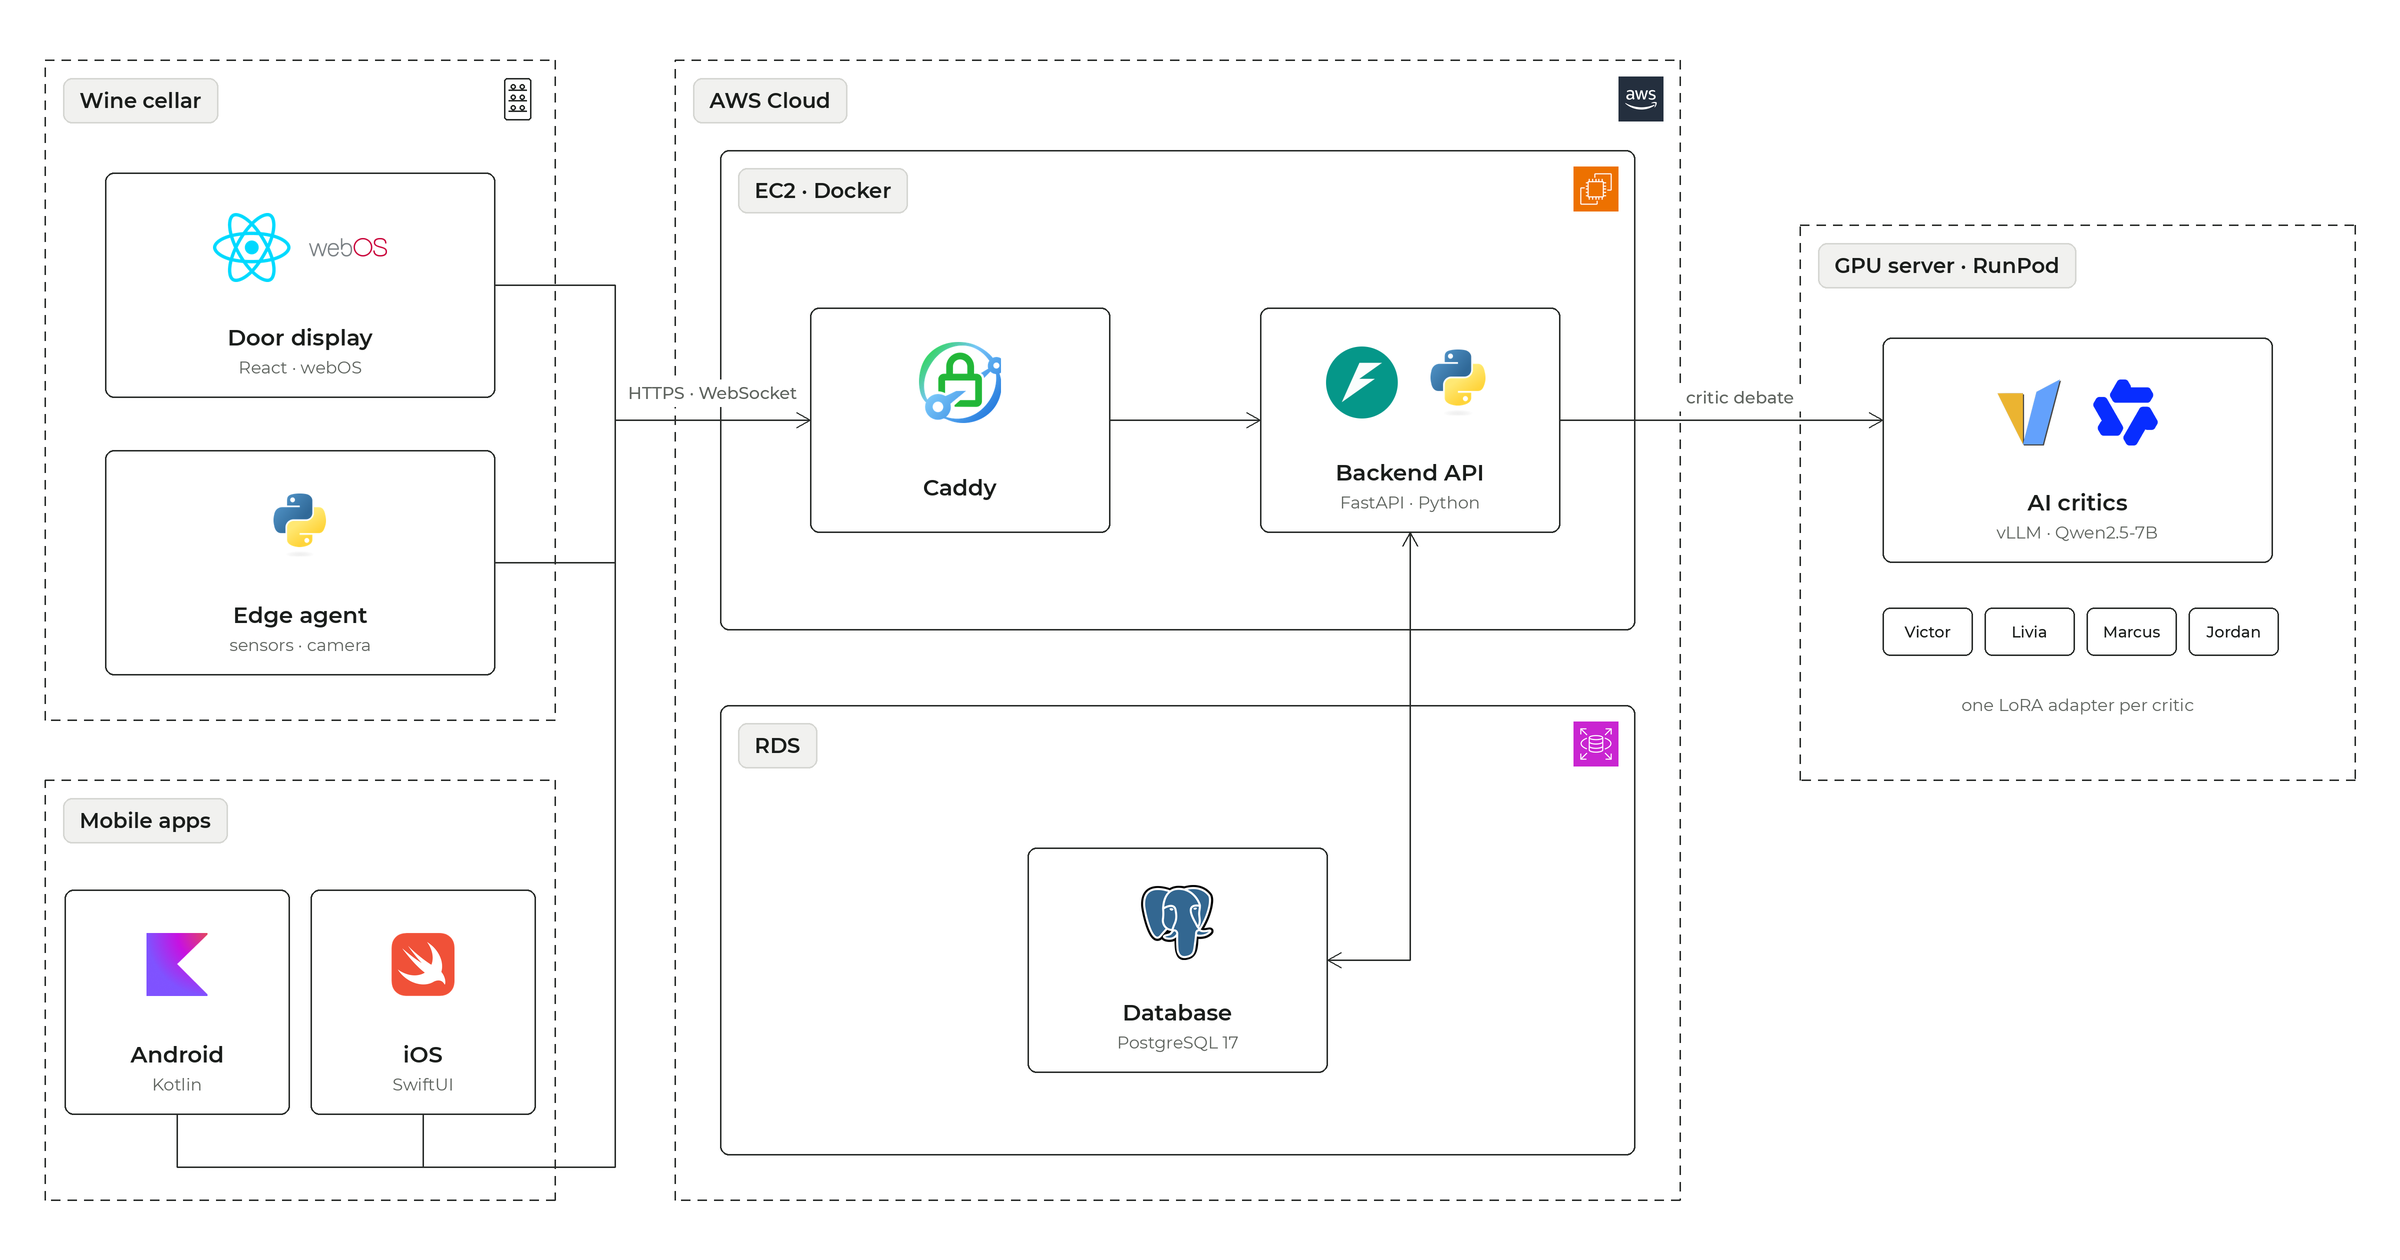
\includegraphics[width=\textwidth]{images/architecture-light.png}
\caption{Overall system architecture. Clients reach the cloud only through Caddy; the backend calls the database, Amazon Rekognition, WineAPI.io, and the RunPod GPU server (purple), where an AI gateway adds evidence before vLLM serves the four critic adapters on one shared base model.}
\label{fig:architecture}
\end{figure*}

\section{Architecture Design \& Implementation}

\subsection{Overall Architecture}
Fig.~\ref{fig:architecture} shows the system. It follows a thin-appliance, smart-cloud design with four parts:
\begin{itemize}
    \item \textbf{Cellar appliance:} the door display (a web application on webOS) and the edge agent, which pairs the cellar with an account and sends sensor readings and cellar scans. Neither runs AI models locally.
    \item \textbf{Cloud backend (AWS):} one FastAPI service that holds all business logic and data (Amazon RDS for PostgreSQL) and is shared by every client.
    \item \textbf{Mobile applications:} native Android and iOS apps that use the same API as the door.
    \item \textbf{AI and data services:} the critic models (an AI gateway and vLLM with four LoRA adapters on a RunPod GPU), Amazon Rekognition for reading label photos, and WineAPI.io for market prices. Only the backend calls them; clients never do, so keys and credentials stay on the server.
\end{itemize}



\subsection{Communication Protocols}
\begin{itemize}
    \item \textbf{REST over HTTPS (client to cloud):} all reads and writes use JSON over HTTPS. Users authenticate with an opaque bearer token; appliances use a separate device token that only allows telemetry and detections for their own cellar.
    \item \textbf{WebSocket (cloud to clients):} after every change the backend sends a short ``changed'' message to all open connections of that owner, and each client reloads the affected data. This keeps the door, Android, and iOS in sync within about a second; polling remains as a fallback.
    \item \textbf{Server-Sent Events (AI answers):} critic debates and recommendations are streamed token by token, so the first words appear while the model is still generating.
    \item \textbf{Device pairing:} a new appliance registers itself and shows a 6-digit code; the owner enters the code in an app, and the appliance then receives its device token.
    \item \textbf{OpenAI-compatible API (backend to GPU server):} the backend sends chat requests with the adapter name as the model, authenticated with a bearer key and streamed; a gateway on the GPU server adds the retrieved evidence before passing the request to vLLM.
    \item \textbf{AWS SDK over HTTPS (backend to Amazon Rekognition):} label photos are sent to the DetectText operation; the EC2 instance's IAM role provides the credentials.
    \item \textbf{REST over HTTPS (backend to WineAPI.io):} price lookups with an API key, made only by the background refresh, never during a client request.
\end{itemize}

\subsection{Directory Organization}
The repository is one monorepo (Table~\ref{tab:directories}); Tables~\ref{tab:dir-backend}--\ref{tab:dir-ai} list the source files of each module.

\par\smallskip
\noindent\begin{minipage}{\columnwidth}
\centering
\refstepcounter{table}\label{tab:directories}
{\footnotesize TABLE \Roman{table}. \textit{Directory Organization}\par}
\smallskip
\footnotesize
\setlength{\tabcolsep}{3pt}
\renewcommand{\arraystretch}{1.05}
\begin{tabularx}{\columnwidth}{|>{\raggedright\arraybackslash}p{0.5\columnwidth}|Y|}
\hline
\multicolumn{1}{|c|}{Directory} & \multicolumn{1}{c|}{Contents} \\
\hline \texttt{backend/} & Cloud backend shared by all clients, with tests \\
\hline \texttt{webos/wine-cellar-display/} & Door display, packaged for webOS \\
\hline \texttt{webos/edge/} & Edge agent (appliance link to the cloud) \\
\hline \texttt{mobile/Kotlin/} & Android application \\
\hline \texttt{mobile/ios/} & iOS application \\
\hline \texttt{AI-7B/} & Critic LoRAs: data, training, evaluation, gateway \\
\hline \texttt{deploy/} & Production deployment (Docker Compose, Caddy) \\
\hline \texttt{documents/} & Paper, requirement coverage, figures \\
\hline \texttt{.github/workflows/} & Continuous integration (GitHub Actions) \\
\hline
\end{tabularx}
\end{minipage}\par\smallskip

\par\smallskip
\noindent\begin{minipage}{\columnwidth}
\centering
\refstepcounter{table}\label{tab:dir-backend}
{\footnotesize TABLE \Roman{table}. \textit{Directory Organization -- Backend (Module 1)}\par}
\smallskip
\footnotesize
\setlength{\tabcolsep}{3pt}
\renewcommand{\arraystretch}{1.05}
\begin{tabularx}{\columnwidth}{|>{\raggedright\arraybackslash}p{0.5\columnwidth}|Y|}
\hline
\textbf{Directory} & \textbf{File Name} \\
\hline \texttt{backend/} & Dockerfile\newline requirements.txt\newline .env.example \\
\hline \texttt{backend/app/} & main.py\newline routes.py\newline devserver.py\newline config.py\newline common.py\newline db.py\newline live.py \\
\hline \texttt{backend/app/ (accounts)} & accounts.py\newline security.py\newline legal.py\newline mailer.py \\
\hline \texttt{backend/app/ (inventory)} & inventory.py\newline geometry.py\newline vision.py\newline labels.py\newline devices.py\newline simulator.py\newline catalog.py \\
\hline \texttt{backend/app/ (AI and data)} & services.py\newline tasting.py\newline llm.py\newline market.py\newline news.py \\
\hline \texttt{backend/tests/} & conftest.py\newline test\_auth.py\newline test\_account.py\newline test\_security.py\newline test\_inventory.py\newline test\_geometry.py\newline test\_vision.py\newline test\_labels.py\newline test\_devices.py\newline test\_environment.py\newline test\_ai.py\newline test\_market.py \\
\hline
\end{tabularx}
\end{minipage}\par\smallskip

\par\smallskip
\noindent\begin{minipage}{\columnwidth}
\centering
\refstepcounter{table}\label{tab:dir-display}
{\footnotesize TABLE \Roman{table}. \textit{Directory Organization -- Door Display (Module 2)}\par}
\smallskip
\footnotesize
\setlength{\tabcolsep}{3pt}
\renewcommand{\arraystretch}{1.05}
\begin{tabularx}{\columnwidth}{|>{\raggedright\arraybackslash}p{0.5\columnwidth}|Y|}
\hline
\textbf{Directory} & \textbf{File Name} \\
\hline \texttt{wine-cellar-display/} & index.html\newline vite.config.ts \\
\hline \texttt{wine-cellar-display/src/} & App.tsx\newline main.tsx\newline api.ts\newline hooks.ts\newline useStream.ts\newline saver.ts\newline types.ts\newline theme.ts\newline styles.css \\
\hline \texttt{src/views/} & Login.tsx\newline Inventory.tsx\newline WineDetails.tsx\newline Sommelier.tsx\newline Briefing.tsx\newline Value.tsx\newline Profile.tsx \\
\hline \texttt{src/components/} & CellarView.tsx\newline CellarStatus.tsx\newline CellarsSettings.tsx\newline ReviewDetection.tsx\newline BottleForm.tsx\newline Debate.tsx\newline StreamOutput.tsx\newline FeaturedBottle.tsx\newline Charts.tsx\newline ClimateHistory.tsx\newline ClimateSettings.tsx\newline Notifications.tsx\newline Consents.tsx\newline Header.tsx\newline ScreenSaver.tsx \\
\hline \texttt{src/sommelier/} & TastingView.tsx\newline NewTasting.tsx\newline Personas.tsx \\
\hline \texttt{scripts/} & webos.mjs \\
\hline \texttt{tests/} & api.test.ts\newline sommelier.test.ts\newline saver.test.ts \\
\hline
\end{tabularx}
\end{minipage}\par\smallskip

\par\smallskip
\noindent\begin{minipage}{\columnwidth}
\centering
\refstepcounter{table}\label{tab:dir-android}
{\footnotesize TABLE \Roman{table}. \textit{Directory Organization -- Android App (Module 3); \texttt{omnicave/} = \texttt{mobile/Kotlin/app/src/main/java/com/example/omnicave}}\par}
\smallskip
\footnotesize
\setlength{\tabcolsep}{3pt}
\renewcommand{\arraystretch}{1.05}
\begin{tabularx}{\columnwidth}{|>{\raggedright\arraybackslash}p{0.5\columnwidth}|Y|}
\hline
\textbf{Directory} & \textbf{File Name} \\
\hline \texttt{omnicave/} & MainActivity.kt \\
\hline \texttt{omnicave/data/} & Api.kt\newline Models.kt\newline Session.kt \\
\hline \texttt{omnicave/ui/auth/} & AuthScreens.kt \\
\hline \texttt{omnicave/ui/main/} & MainScreen.kt \\
\hline \texttt{omnicave/ui/cellar/} & CellarScreen.kt\newline Cellar3D.kt \\
\hline \texttt{omnicave/ui/inventory/} & InventoryScreen.kt \\
\hline \texttt{omnicave/ui/wine/} & WineDetailsScreen.kt\newline BottleFormScreen.kt \\
\hline \texttt{omnicave/ui/sommelier/} & SommelierScreen.kt\newline TastingScreen.kt\newline PersonasScreen.kt \\
\hline \texttt{omnicave/ui/briefing/} & BriefingScreen.kt \\
\hline \texttt{omnicave/ui/value/} & ValueScreen.kt \\
\hline \texttt{omnicave/ui/profile/} & ProfileScreen.kt\newline ClimateSettings.kt \\
\hline \texttt{omnicave/ui/components/} & Controls.kt\newline Charts.kt\newline Consents.kt\newline Icons.kt \\
\hline \texttt{omnicave/ui/theme/} & Color.kt\newline Theme.kt\newline Type.kt \\
\hline \texttt{app/src/test/.../data/} & ModelsTest.kt \\
\hline
\end{tabularx}
\end{minipage}\par\smallskip

\par\smallskip
\noindent\begin{minipage}{\columnwidth}
\centering
\refstepcounter{table}\label{tab:dir-ios}
{\footnotesize TABLE \Roman{table}. \textit{Directory Organization -- iOS App (Module 3)}\par}
\smallskip
\footnotesize
\setlength{\tabcolsep}{3pt}
\renewcommand{\arraystretch}{1.05}
\begin{tabularx}{\columnwidth}{|>{\raggedright\arraybackslash}p{0.5\columnwidth}|Y|}
\hline
\textbf{Directory} & \textbf{File Name} \\
\hline \texttt{mobile/ios/} & Package.swift \\
\hline \texttt{mobile/ios/OmniCave/} & OmniCaveApp.swift\newline AppModel.swift\newline Services.swift\newline BackendModels.swift\newline Models.swift\newline Views.swift \\
\hline \texttt{mobile/ios/OmniCaveTests/} & APIClientTests.swift \\
\hline
\end{tabularx}
\end{minipage}\par\smallskip

\par\smallskip
\noindent\begin{minipage}{\columnwidth}
\centering
\refstepcounter{table}\label{tab:dir-ai}
{\footnotesize TABLE \Roman{table}. \textit{Directory Organization -- Edge, AI and Deployment (Modules 4--6)}\par}
\smallskip
\footnotesize
\setlength{\tabcolsep}{3pt}
\renewcommand{\arraystretch}{1.05}
\begin{tabularx}{\columnwidth}{|>{\raggedright\arraybackslash}p{0.5\columnwidth}|Y|}
\hline
\textbf{Directory} & \textbf{File Name} \\
\hline \texttt{webos/edge/} & edge\_agent.py \\
\hline \texttt{AI-7B/} & build\_pool.py\newline build\_xwines.py\newline evidence7b.py\newline generate.py\newline verify7b.py\newline train.py\newline eval7b.py\newline serve\_check7b.py\newline gateway.py\newline prompts.py\newline check\_prompt\_sync.py \\
\hline \texttt{AI-7B/pod/} & setup.sh\newline run.sh\newline wait.sh\newline train\_all.sh\newline rebalance.py\newline serve.sh\newline serve\_check.sh \\
\hline \texttt{deploy/} & docker-compose.yml\newline Caddyfile\newline .env.production.example \\
\hline
\end{tabularx}
\end{minipage}\par\smallskip

\subsection{Module 1: Cloud Backend}
\textbf{Purpose.} Keep all business logic and data in one cloud service, so that the door, the Android app, and the iOS app behave identically and the cellar appliance can stay a thin client.

\textbf{Functionality.}
\begin{enumerate}
    \item \textbf{Accounts and privacy:} sign-up with the 19+ age check and separate PIPA consents, login with a username or email, opaque bearer tokens, optional email codes, data export, and account deletion.
    \item \textbf{Inventory and geometry:} cellars, removable racks, climate zones, and bottles in centimeter coordinates; free placement with a gravity rule for stacked bottles; search across all cellars.
    \item \textbf{Vision:} label photos become wine details (Amazon Rekognition and a catalog match); cellar scans are reconciled into new, moved, hidden, and removed bottles; uncertain results wait in a review queue.
    \item \textbf{Appliances and climate:} 6-digit pairing, device tokens limited to their own cellar, telemetry, and alerts for out-of-range or silent sensors.
    \item \textbf{AI and data:} the critic table, pairing, recommendations, and the daily briefing; one switch between the mock provider and the GPU server; market prices from WineAPI.io and news from RSS feeds.
    \item \textbf{Live sync:} after every change a short message goes over WebSocket to all of the owner's open clients, which then reload the affected data.
\end{enumerate}

\textbf{Location of source code.} \url{https://github.com/enkhbold0519/omnicave/tree/main/backend}

\textbf{Class components.}
\begin{itemize}
    \item \texttt{main.py}: FastAPI application: mounts the route table, the WebSocket endpoint, and starts the background loops.
    \item \texttt{routes.py}: one framework-independent table of every endpoint (method, path, service function, access level); also served by the standard-library \texttt{devserver.py} used in the tests.
    \item \texttt{config.py, db.py, common.py}: settings from the environment; one SQL layer that runs the same statements on SQLite and PostgreSQL, with migrations; shared helpers and the notification function.
    \item \texttt{security.py, accounts.py, legal.py, mailer.py}: salted PBKDF2-SHA256 passwords~\cite{pbkdf2} and hashed tokens~\cite{bearer}; sign-up rules and email codes; consent list and policy versions; email sending.
    \item \texttt{inventory.py, geometry.py}: cellars, racks, zones, and bottles; free-spot search, snapping to a rack, stacking levels, and settling when a supporting bottle is removed.
    \item \texttt{vision.py, labels.py}: scan reconciliation in the style of tracking-by-detection~\cite{sort} with a 2.5 cm noise tolerance; label photo to wine details.
    \item \texttt{devices.py, simulator.py}: appliance registration, pairing, and telemetry; background loop for simulated sensors, climate alerts, drinking-window notices, and the daily briefing.
    \item \texttt{services.py, tasting.py, llm.py}: recommendations, briefing, and value; the critic table, deciding per turn between a critic's LoRA and the base model; streaming client for the LLM server with a silent mock fallback.
    \item \texttt{market.py, news.py, catalog.py}: daily-cached WineAPI.io prices; RSS news ranked against the owner's cellar; reference wine catalog.
    \item \texttt{live.py}: WebSocket hub that keeps the open connections per user and sends the change messages.
\end{itemize}

\textbf{Technologies.} Python 3.12, FastAPI, Uvicorn, psycopg, boto3 (AWS SDK), PostgreSQL 17 (Amazon RDS), SQLite, Docker, pytest.

\subsection{Module 2: Door Display}
\textbf{Purpose.} Turn the transparent cellar door into the main interface: show what is inside and where, and bring the critics and the cellar's data to the appliance itself.

\textbf{Functionality.}
\begin{enumerate}
    \item \textbf{Cellar:} a to-scale door view and a rotatable 3D view of racks and bottles, with the climate of each zone; Find highlights one bottle in both views.
    \item \textbf{Inventory:} search across cellars with filters, bottle details with drinking window and value, manual add, edit, move, open, and remove.
    \item \textbf{Recognition review:} new bottles from label photos or scans wait for the owner to confirm or correct them.
    \item \textbf{Critics, briefing, and value:} the critic tasting table and the owner's own critics, the daily briefing, and the collection value.
    \item \textbf{Always-on door:} a fixed 1080$\times$1920 portrait canvas, scaled and rotated for landscape panels, with black backgrounds because black pixels are see-through on a transparent OLED; a screen saver and a night mode.
    \item \textbf{Offline:} the last data is cached and changes made offline are queued and sent once the connection returns.
\end{enumerate}

\textbf{Location of source code.} \url{https://github.com/enkhbold0519/omnicave/tree/main/webos/wine-cellar-display}

\textbf{Class components.}
\begin{itemize}
    \item \texttt{App.tsx}: the five main pages, the portrait canvas, login state, live-sync connection, and the screen-saver timer.
    \item \texttt{api.ts, hooks.ts, useStream.ts}: REST client with offline cache and write queue, cleared at logout; polling and draft-saving hooks; reader for streamed AI answers.
    \item \texttt{views/}: one file per page: Login (sign-up with consents), Inventory, WineDetails, Sommelier, Briefing, Value, Profile.
    \item \texttt{components/CellarView.tsx}: door view and 3D view, highlighting, and placing a bottle by touch.
    \item \texttt{components/ReviewDetection.tsx, BottleForm.tsx}: confirm or correct a recognized bottle; the manual add and edit form.
    \item \texttt{components/ScreenSaver.tsx, FeaturedBottle.tsx}: the two screen-saver styles and night mode.
    \item \texttt{components/ClimateHistory.tsx, ClimateSettings.tsx, Notifications.tsx}: zone charts, limits and alert delay, and the notification list.
    \item \texttt{sommelier/}: the tasting table, starting a tasting, creating critics, and the score and verdict logic (\texttt{model.ts}).
    \item \texttt{scripts/webos.mjs, tests/}: packaging, installing, and launching on webOS; Vitest unit tests.
\end{itemize}

\textbf{Technologies.} React 19, TypeScript 5.9, Vite 7 (one IIFE bundle, because webOS loads apps from \texttt{file://}), webOS OSE 2.28, Vercel, Vitest.

\begin{figure}[htbp]
\centering
\shot{cellar-door.jpg}{(a) Door view}\hfill\shot{cellar-3d.jpg}{(b) 3D view}
\caption{Door Display: Door View and 3D View}
\label{fig:display-home}
\end{figure}

\subsection{Module 3: Mobile Applications}
\textbf{Purpose.} Give owners the same control of their cellars away from the door, natively on Android and iOS.

\textbf{Functionality.}
\begin{enumerate}
    \item \textbf{Accounts:} sign-up with consents and the age check, login, and privacy settings.
    \item \textbf{Cellar and inventory:} cellar map, search, bottle details, and adding a bottle from a label photo.
    \item \textbf{Climate and notifications:} zone readings, limits, remote target changes, and the notification list.
    \item \textbf{Critics, briefing, and value:} the tasting table with streamed answers, the daily briefing, and the collection value.
    \item \textbf{Live sync:} both apps listen on the WebSocket, so a change on the door or the other phone appears at once.
\end{enumerate}

\textbf{Location of source code.} \url{https://github.com/enkhbold0519/omnicave/tree/main/mobile}

\textbf{Class components.}
\begin{itemize}
    \item \texttt{Android data/Api.kt}: the one place that talks to the backend: REST, streamed answers, label-photo upload, and the WebSocket listener.
    \item \texttt{Android data/Models.kt, Session.kt}: the backend's JSON shapes; the login token kept on the phone.
    \item \texttt{Android ui/}: one file per screen (main, cellar with 3D view, inventory, wine details and form, sommelier, briefing, value, profile and climate), shared controls and theme.
    \item \texttt{Android src/test/}: unit tests for the JSON models.
    \item \texttt{iOS Services.swift}: backend client: REST, streaming, and live updates.
    \item \texttt{iOS AppModel.swift, BackendModels.swift}: app state and actions; the backend's JSON shapes.
    \item \texttt{iOS Views.swift, OmniCaveApp.swift}: all SwiftUI screens; app entry point and server address.
    \item \texttt{iOS OmniCaveTests/}: unit tests for the API client.
\end{itemize}

\textbf{Technologies.} Kotlin 2.2, Jetpack Compose, OkHttp; Swift, SwiftUI, URLSession, Keychain.

\subsection{Module 4: Edge Agent and Cellar Simulation}
\textbf{Purpose.} Stand in for the appliance hardware we do not have, using exactly the interface a real cellar would use.

\textbf{Functionality.}
\begin{enumerate}
    \item \textbf{Pairing:} the agent registers the appliance, shows the 6-digit code, and receives its device token once the owner pairs it.
    \item \textbf{Telemetry:} temperature and humidity readings are sent at a fixed interval.
    \item \textbf{Camera frames:} frames from a folder of images or a webcam can be uploaded for analysis in the cloud.
    \item \textbf{Simulation:} because no cellar, camera, or sensors were available, the backend simulates climate readings (including faults such as a disconnected sensor) and cellar scans in which bottles are added, moved, stacked, hidden, or removed; the scans go through the same reconciliation as real detections.
\end{enumerate}

\textbf{Location of source code.} \url{https://github.com/enkhbold0519/omnicave/tree/main/webos/edge}

\textbf{Class components.}
\begin{itemize}
    \item \texttt{edge\_agent.py}: pairing, telemetry loop, and frame upload.
    \item \texttt{backend/app/simulator.py}: climate readings, fault injection, and the scheduled alerts.
    \item \texttt{backend/app/vision.py (simulate\_scan)}: simulated cellar scans with a known ground truth.
\end{itemize}

\textbf{Technologies.} Python standard library (OpenCV only for the optional webcam).

\subsection{Module 5: AI Critic Engine}
\textbf{Purpose.} Let four critics with clearly different judgment debate any bottle on the door, while every fact they state (scores, prices, drinking windows, crowd ranks) comes from real data. The critics are the feature that turns the cellar from storage into a sommelier.

\textbf{Design decision: adapters, not prompts.} We first gave each critic's philosophy to the base model as a prompt. It wrote fluent text, but every critic fell back to the same generic voice: only 0--28\% of answers passed all checks, and three of the four critics never used their own scoring scale (Table~\ref{tab:lora-eval}). A larger cloud model would cost more per request and still drift. Instead, each critic is a small LoRA adapter~\cite{lora} on one shared Qwen2.5-7B-Instruct base~\cite{qwen25}: the adapter carries the critic's voice and way of arguing, and the facts are retrieved at answer time~\cite{rag}, which keeps the model from inventing them~\cite{hallucination}. Table~\ref{tab:critics} lists the four critics.

\par\smallskip
\noindent\begin{minipage}{\columnwidth}
\centering
\refstepcounter{table}\label{tab:critics}
{\footnotesize TABLE \Roman{table}. \textit{The Four Critics}\par}
\smallskip
\footnotesize
\setlength{\tabcolsep}{3pt}
\renewcommand{\arraystretch}{1.1}
\begin{tabularx}{\columnwidth}{|>{\raggedright\arraybackslash}p{0.2\columnwidth}|Y|>{\raggedright\arraybackslash}p{0.23\columnwidth}|}
\hline
\multicolumn{1}{|c|}{Critic} & \multicolumn{1}{c|}{How they judge} & \multicolumn{1}{c|}{Verdict on} \\
\hline Victor Hale, 100-point power critic & rewards concentration, ripeness, and new-oak polish; openly prefers Bordeaux and the Rh\^one & a 2--3 point range, e.g., ``93--95 points'' \\
\hline Livia Moretti, fruit-quality analyst & judges the richness of the fruit against acidity and tannin; prefers Italian wine & a fruit quality index, e.g., ``FQI 1.6'' \\
\hline Marcus Reed, value-first editor & weighs quality against price, only within the same region and grape & a score and a value grade, e.g., ``91 points, B+'' \\
\hline Jordan Reyes, crowd-taste tracker & speaks for everyday drinkers from community ratings, ranked only against the same region and grape & a peer rank, e.g., ``top 15\% of 188'' \\
\hline
\multicolumn{3}{p{0.95\columnwidth}}{\scriptsize All four are fictional; real critics, magazines, and review sites are never named, and the verifier rejects any turn that does.}
\end{tabularx}
\end{minipage}\par\smallskip

\textbf{Functionality.}
\begin{enumerate}
    \item \textbf{Evidence retrieval:} a pool of 440 wines with real, aggregated evidence: critic score ranges, prices, drinking windows, and crowd ratings from the open X-Wines dataset~\cite{xwines}. No review text or reviewer names are kept. At answer time the evidence for the wine and the critic is added to the prompt, so new wines need no retraining.
    \item \textbf{Training data:} a larger teacher model (Qwen2.5-32B) writes four candidate debate turns per prompt, a form of distillation into the small model~\cite{distill,selfinstruct}. A rule-based verifier keeps a turn only if every year, price, and tasting note appears in the evidence, the critic's own scale is used, the length fits, and no real name appears; about 1,000 verified turns per critic remain (Table~\ref{tab:ai-data}).
    \item \textbf{Training:} one rank-16 LoRA per critic (3 epochs, 3--11 minutes each on one GPU); the evaluation loss fell by about 55--60\% for every critic.
    \item \textbf{Serving:} vLLM~\cite{vllm} keeps one base model in GPU memory and applies the requested adapter per request, so four critics cost little more than one model~\cite{slora,punica}. A gateway in front of vLLM finds the wine and the critic in each request and appends their evidence.
    \item \textbf{Use in the backend:} when the owner starts a tasting on a wine, each built-in critic answers with its own adapter and the exact prompt it was trained on, and its score and peak year become a badge in the apps. As soon as the owner joins the conversation, and for questions such as ``what should I open tonight?'' or for critics the owner created, the base model answers with a prompt that describes the critic and the owner's cellar and taste. Each critic also remembers what it has learned about the owner.
    \item \textbf{Fallback:} the GPU server runs only when needed; if it cannot be reached, the backend streams a short stand-in answer and skips the server for 60 seconds, so the apps never hang.
\end{enumerate}

\begin{figure*}[t]
\centering
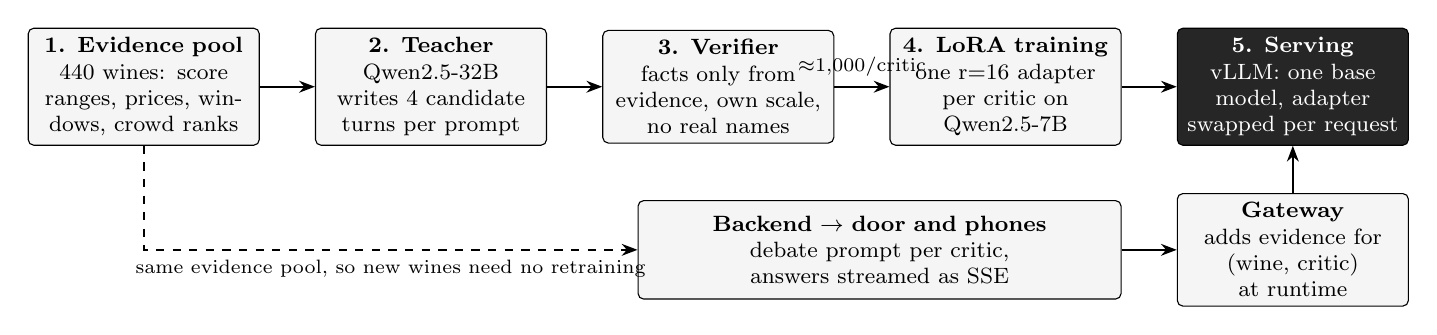
\begin{tikzpicture}[every node/.style={font=\footnotesize}, box/.style={draw, rounded corners=2pt, align=center, text width=2.7cm, minimum height=1.25cm, fill=gray!8}, arr/.style={-{Stealth[length=2mm]}, thick}]
\node[box] (pool) {\textbf{1. Evidence pool}\\440 wines: score ranges, prices, windows, crowd ranks};
\node[box, right=7mm of pool] (teach) {\textbf{2. Teacher}\\Qwen2.5-32B writes 4 candidate turns per prompt};
\node[box, right=7mm of teach] (ver) {\textbf{3. Verifier}\\facts only from evidence, own scale, no real names};
\node[box, right=7mm of ver] (train) {\textbf{4. LoRA training}\\one r=16 adapter per critic on Qwen2.5-7B};
\node[box, right=7mm of train, fill=black!85, text=white] (serve) {\textbf{5. Serving}\\vLLM: one base model, adapter swapped per request};
\draw[arr] (pool) -- (teach);
\draw[arr] (teach) -- (ver);
\draw[arr] (ver) -- node[above, font=\scriptsize]{$\approx$1,000/critic} (train);
\draw[arr] (train) -- (serve);
\node[box, below=6mm of serve, text width=2.7cm] (gw) {\textbf{Gateway}\\adds evidence for (wine, critic) at runtime};
\node[box, left=7mm of gw, text width=5.9cm] (apps) {\textbf{Backend $\rightarrow$ door and phones}\\debate prompt per critic, answers streamed as SSE};
\draw[arr] (apps) -- (gw);
\draw[arr] (gw) -- (serve);
\draw[arr, dashed] (pool.south) |- node[pos=0.75, below, font=\scriptsize]{same evidence pool, so new wines need no retraining} (apps.west);
\end{tikzpicture}
\caption{AI Critic Engine: Training (Top) and Serving (Bottom)}
\label{fig:ai-pipeline}
\end{figure*}

\par\smallskip
\noindent\begin{minipage}{\columnwidth}
\centering
\refstepcounter{table}\label{tab:ai-data}
{\footnotesize TABLE \Roman{table}. \textit{Training Data and Loss per Critic}\par}
\smallskip
\footnotesize
\setlength{\tabcolsep}{3pt}
\begin{tabular}{|l|c|c|c|c|}
\hline
Critic & Verified & Train & Held-out & Eval loss \\
\hline Victor Hale (power) & 1,112 & 1,048 & 64 & 1.59 $\rightarrow$ 0.65 \\
\hline Livia Moretti (fruit) & 1,065 & 1,004 & 61 & 1.72 $\rightarrow$ 0.70 \\
\hline Marcus Reed (value) & 1,060 & 999 & 61 & 1.42 $\rightarrow$ 0.59 \\
\hline Jordan Reyes (crowd) & 892 & 227$^{*}$ & 49 & 1.29 $\rightarrow$ 0.58 \\
\hline
\multicolumn{5}{l}{\scriptsize $^{*}$turns without crowd evidence capped at 35\%, so the critic does not learn to guess.}
\end{tabular}
\end{minipage}\par\smallskip
\textbf{Evaluation.} Both conditions were tested on held-out wines that never appeared in training: up to 40 prompts per critic, the same prompt and the same retrieved evidence, sampled at temperature 0.8. An answer passes only if it uses the critic's own scale and no other critic's scale, has two to three sentences, states only years, prices, and tasting notes found in the evidence, and names no real critic. The adapters passed all checks in 98--100\% of answers, against 0--28\% for the base model (Fig.~\ref{fig:ai-results}, Table~\ref{tab:lora-eval}). Both conditions stayed grounded in the evidence; the difference lies entirely in keeping each critic's voice and scale. An earlier study on a 1.5B-parameter model showed that a rank-4 adapter already learned the style but made 2 factual slips in 40 answers, so rank 16 was used here.

\begin{figure}[htbp]
\centering
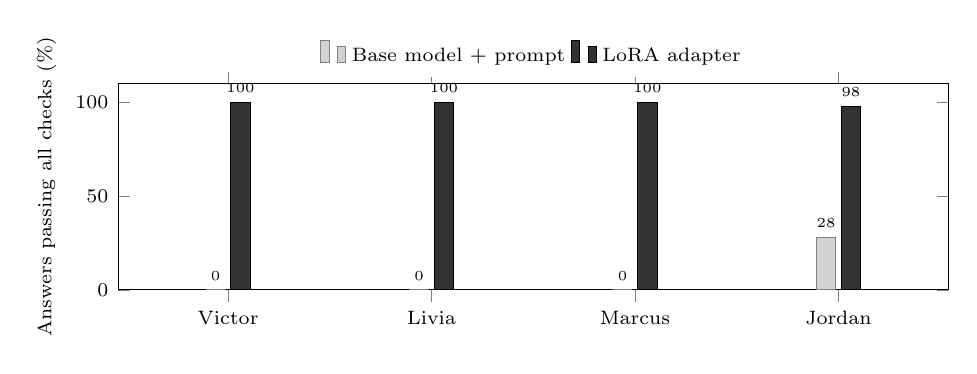
\begin{tikzpicture}
\begin{axis}[ybar, width=\columnwidth, height=4.2cm, bar width=7pt, ymin=0, ymax=110, ylabel={Answers passing all checks (\%)}, ylabel style={font=\scriptsize}, symbolic x coords={Victor,Livia,Marcus,Jordan}, xtick=data, tick label style={font=\scriptsize}, nodes near coords, nodes near coords style={font=\tiny}, legend style={font=\scriptsize, at={(0.5,1.03)}, anchor=south, legend columns=2, draw=none}, enlarge x limits=0.18]
\addplot[fill=gray!35, draw=gray] coordinates {(Victor,0) (Livia,0) (Marcus,0) (Jordan,28)};
\addplot[fill=black!80, draw=black] coordinates {(Victor,100) (Livia,100) (Marcus,100) (Jordan,98)};
\legend{Base model + prompt, LoRA adapter}
\end{axis}
\end{tikzpicture}
\caption{Critic Checks on Held-Out Wines (n = 40 per Critic)}
\label{fig:ai-results}
\end{figure}

\par\smallskip
\noindent\begin{minipage}{\columnwidth}
\centering
\refstepcounter{table}\label{tab:lora-eval}
{\footnotesize TABLE \Roman{table}. \textit{Checks Passed on Held-Out Wines (n = 40 each), Base / LoRA}\par}
\smallskip
\scriptsize
\setlength{\tabcolsep}{2.5pt}
\begin{tabular}{|l|c|c|c|c|}
\hline
Critic & Own scale & Format & Grounded & All checks \\
\hline Victor Hale & 0 / 100 & 15 / 100 & 100 / 100 & \textbf{0 / 100} \\
\hline Livia Moretti & 0 / 100 & 10 / 100 & 100 / 100 & \textbf{0 / 100} \\
\hline Marcus Reed & 0 / 100 & 12 / 100 & 100 / 100 & \textbf{0 / 100} \\
\hline Jordan Reyes & 85 / 100 & 30 / 98 & 100 / 100 & \textbf{28 / 98} \\
\hline
\multicolumn{5}{p{0.95\columnwidth}}{\scriptsize Values in \%. Format: 2--3 sentences. Grounded: every year, price, and tasting note appears in the evidence.}
\end{tabular}
\end{minipage}\par\smallskip
\textbf{Example.} Three critics on a held-out wine (Dona Maria J\'ulio Bastos Red 2014), generated by the adapters:
\begin{quote}\footnotesize
\textbf{Victor Hale:} ``\ldots showcases a juicy and rich profile, aligning well with the concentrated and structured style I favor. I would score this wine 91--93 points.''\\
\textbf{Livia Moretti:} ``\ldots I find the tannins to be a bit hard, which detracts from the fruit quality. I give it an FQI 1.6.''\\
\textbf{Marcus Reed:} ``This \ldots earns 90 points and a value grade B+ \ldots offers good value at \$15.''
\end{quote}
The same bottle receives three different verdicts on three different scales, each defensible from the same evidence; this disagreement is what the tasting table shows the owner.

\textbf{Serving performance.} Table~\ref{tab:serving} shows that a critic starts speaking within the 1.5-second target of the performance requirement, even when the request travels from the door to the cloud and on to the GPU server. \todo{Sungbin: confirm numbers}

\par\smallskip
\noindent\begin{minipage}{\columnwidth}
\centering
\refstepcounter{table}\label{tab:serving}
{\footnotesize TABLE \Roman{table}. \textit{Serving Measurements}\par}
\smallskip
\footnotesize
\setlength{\tabcolsep}{3pt}
\renewcommand{\arraystretch}{1.1}
\begin{tabularx}{\columnwidth}{|Y|>{\raggedright\arraybackslash}p{0.33\columnwidth}|}
\hline
\multicolumn{1}{|c|}{Measurement} & \multicolumn{1}{c|}{Result} \\
\hline First token per critic, measured on the GPU server & 0.05--0.07 s \\
\hline First token at the cloud backend, through the RunPod proxy (NVIDIA A40) & 1.0--1.2 s (target: 1.5 s) \\
\hline Served prompts identical to the training prompts (gateway check) & 235 of 235 \\
\hline Total GPU cost (data generation, training, evaluation) & \$4.45 \\
\hline
\end{tabularx}
\end{minipage}\par\smallskip

\textbf{Limitations.} The critics answer in English, because the adapters were trained on English data only; the base-model features follow the owner's language. Crowd evidence exists only for part of the wines, so Jordan Reyes says so instead of ranking a bottle without data. The GPU server is rented on demand, so outside test and demo sessions the critics use the stand-in answer.

\textbf{Location of source code.} \url{https://github.com/enkhbold0519/omnicave/tree/main/AI-7B}

\textbf{Class components.}
\begin{itemize}
    \item \texttt{build\_xwines.py, build\_pool.py}: build the evidence pool from open data: score ranges, prices, drinking windows, and crowd ratings for 440 wines.
    \item \texttt{evidence7b.py, prompts.py}: turn a pool row into each critic's evidence block; the debate prompt, identical to the backend's.
    \item \texttt{generate.py, verify7b.py}: teacher generation of candidate turns; the rule-based checks that keep only grounded, in-character turns.
    \item \texttt{train.py, eval7b.py}: LoRA training with PEFT~\cite{peft}; base-versus-LoRA evaluation on held-out wines.
    \item \texttt{gateway.py}: the retrieval step in front of vLLM: finds the wine and critic in a request and appends the evidence.
    \item \texttt{serve\_check7b.py, check\_prompt\_sync.py}: measure the first-token time of a running server; fail if the backend prompt drifts from the training prompt.
    \item \texttt{pod/}: scripts that set up the GPU pod, train all critics, and start serving.
\end{itemize}

\textbf{Technologies.} PyTorch, Hugging Face Transformers~\cite{transformers} and PEFT~\cite{peft}, vLLM~\cite{vllm}, RunPod GPUs. Taken from: the base and teacher models are open-weight Qwen2.5 (Apache-2.0); everything else, including the data pipeline, verifier, and gateway, was written by the team.

\subsection{Module 6: Deployment}
\textbf{Purpose.} Run the shared backend reliably and cheaply for development and demonstrations, and check every change automatically.

\textbf{Functionality.}
\begin{enumerate}
    \item \textbf{Server:} Docker Compose runs the backend and Caddy on one EC2 instance; Caddy obtains HTTPS certificates automatically and passes WebSocket and streamed answers through.
    \item \textbf{Data:} the database is a private Amazon RDS instance with automated daily backups, so the server itself holds no data and can be replaced.
    \item \textbf{Display hosting:} the door display is hosted on Vercel and packaged as an \texttt{.ipk} for webOS.
    \item \textbf{GPU on demand:} the critic server is started only for tests and demonstrations; otherwise the backend uses the mock provider.
    \item \textbf{Continuous integration:} every push runs the test suites and builds (Section~\ref{sec:testing}).
\end{enumerate}

\textbf{Location of source code.} \url{https://github.com/enkhbold0519/omnicave/tree/main/deploy}

\textbf{Class components.}
\begin{itemize}
    \item \texttt{docker-compose.yml}: the API and Caddy containers, their settings, and the certificate volume.
    \item \texttt{Caddyfile}: HTTPS and reverse proxy to the API.
    \item \texttt{.env.production.example}: template for the server settings (database, AI, prices, label reading, email).
    \item \texttt{backend/Dockerfile}: the Python 3.12 image of the backend.
    \item \texttt{.github/workflows/ci.yml}: the five CI jobs.
\end{itemize}

\textbf{Technologies.} AWS EC2 (t3.small), Amazon RDS for PostgreSQL 17, Amazon Rekognition, Docker, Caddy, Vercel, RunPod, GitHub Actions. The AWS resources run in the Sydney region (ap-southeast-2), which our AWS plan is limited to; a production deployment would run in the LG Datacenter or a Korean region.

\subsection{Testing and Continuous Integration}\label{sec:testing}
Every push and pull request runs five GitHub Actions jobs (Table~\ref{tab:tests}). The backend suite starts the real API on a temporary database and calls it over HTTP, so the tests exercise the same routes as the apps; it runs once on SQLite and once on PostgreSQL 17, because the two databases differ in small ways that only show up at run time. A further job checks that the debate prompt in the backend is still identical to the one the LoRA adapters were trained on.

\par\smallskip
\noindent\begin{minipage}{\columnwidth}
\centering
\refstepcounter{table}\label{tab:tests}
{\footnotesize TABLE \Roman{table}. \textit{Automated Tests}\par}
\smallskip
\footnotesize
\setlength{\tabcolsep}{3pt}
\renewcommand{\arraystretch}{1.05}
\begin{tabularx}{\columnwidth}{|>{\raggedright\arraybackslash}p{0.22\columnwidth}|>{\raggedright\arraybackslash}p{0.10\columnwidth}|Y|}
\hline
\multicolumn{1}{|c|}{Component} & \multicolumn{1}{c|}{Tests} & \multicolumn{1}{c|}{Coverage and where it runs} \\
\hline Backend (pytest) & 42 & Accounts, consents, security, inventory, geometry, vision reconciliation, label reading, devices, climate, AI, market prices; CI on SQLite and PostgreSQL \\
\hline Door display (Vitest) & 18 & Critic score badges and verdict, offline cache and write queue, logout clean-up, sign-up reply, screen saver; CI before every build \\
\hline Android (JUnit) & 11 & JSON models; CI compiles the app \\
\hline iOS (XCTest) & 5 & API client; run in Xcode on macOS \\
\hline AI prompt check & 1 & Served debate prompt equals the training prompt; CI \\
\hline
\end{tabularx}
\end{minipage}\par\smallskip

The tests found real defects: the PostgreSQL job caught a database statement that worked only on SQLite, and the display tests showed that changes queued while offline were sent twice after reconnecting and that a logged-out user's cached data stayed on the door. All three were fixed before submission.

\section{Use Cases}
This section describes the main use cases from the owner's point of view, each linked to the requirement it covers. Screens are from the door display; the phone apps offer the same flows except the screen saver (UC12), which exists only on the door.

\subsection{UC1: Create an Account}
\textbf{Requirement:} User Management \quad \textbf{Actors:} Owner

\textbf{Preconditions:} The app is installed; the owner is 19 or older.

\textbf{Flow:}
\begin{enumerate}
    \item The owner opens Sign up and enters a username, email, password, and birth date; a checklist shows the password rules.
    \item The owner ticks the required consents (or ``Agree to all'') and taps Sign up.
    \item If email verification is on, the owner enters the 6-digit code from the email.
    \item The owner logs in with the username or the email.
\end{enumerate}
\textbf{Postconditions:} The account exists with its consents recorded; the owner sees the main screen.

\begin{figure}[htbp]
\centering
\shot[0.48]{login.jpg}{(a) Log in}\hfill\shot[0.48]{signup.jpg}{(b) Sign up}
\caption{Log In and Sign Up}
\label{fig:uc-signup}
\end{figure}

\subsection{UC2: Connect a New Cellar}
\textbf{Requirement:} Multi-Cellar Management \quad \textbf{Actors:} Owner, cellar appliance

\textbf{Preconditions:} The owner is logged in; the cellar is powered on and online.

\textbf{Flow:}
\begin{enumerate}
    \item The cellar door shows a 6-digit pairing code.
    \item In the app, the owner chooses Add cellar and enters the code and a name.
    \item The cellar appears in the app and on the door, with its racks and zones.
\end{enumerate}
\textbf{Postconditions:} The appliance is linked to the account and starts sending sensor data.

\todo{screenshot from the phone app: Add cellar with the pairing code}

\subsection{UC3: Store a New Bottle}
\textbf{Requirement:} Inventory Mapping \quad \textbf{Actors:} Owner, label recognition (Amazon Rekognition)

\textbf{Preconditions:} A paired cellar.

\textbf{Flow:}
\begin{enumerate}
    \item The owner chooses ``From photo'' in the app and photographs the bottle's front label (in the product, an entry camera at the door takes this photo).
    \item The label text is read in the cloud and matched to a wine; the bottle appears in the review queue with its details, a suggested free spot, and the recognition confidence.
    \item The owner corrects the vintage if needed and confirms.
    \item The owner places the bottle in the suggested spot; it is registered at that position and appears on the door and the phone at the same time.
\end{enumerate}
\textbf{Postconditions:} One new bottle record with a unique serial and a centimeter position.

\begin{figure}[htbp]
\centering
\shot[0.48]{detection.jpg}{(a) New bottle recognized}\hfill\shot[0.48]{review.jpg}{(b) Review and confirm}
\caption{Storing a New Bottle}
\label{fig:uc-review}
\end{figure}

\subsection{UC4: Find a Bottle}
\textbf{Requirement:} Inventory Search \& Visualization \quad \textbf{Actors:} Owner

\textbf{Preconditions:} Bottles stored in one or more cellars.

\textbf{Flow:}
\begin{enumerate}
    \item The owner types ``Pinot'' in the search on the door or the phone, for all cellars.
    \item Results list each bottle with its cellar and rack; selecting one opens its details.
    \item The owner taps Find: the door view marks the bottle with a ring and its name, at its measured position.
    \item Switching to the 3D view shows the same bottle highlighted inside the turning cellar, including bottles stacked on others or in the back row.
\end{enumerate}
\textbf{Postconditions:} The owner knows which cellar, rack, and position to reach for.

\begin{figure}[htbp]
\centering
\shot[0.48]{search.jpg}{(a) Search}\hfill\shot[0.48]{wine-detail.jpg}{(b) Bottle details}\\[6pt]
\shot[0.48]{find-door.jpg}{(c) Found on the door view}\hfill\shot[0.48]{find-3d.jpg}{(d) Found in the 3D view}
\caption{Finding a Bottle}
\label{fig:uc-search}
\end{figure}

\subsection{UC5: Open or Remove a Bottle}
\textbf{Requirement:} Inventory Mapping; AI Recommendations \quad \textbf{Actors:} Owner

\textbf{Preconditions:} The bottle is in the inventory.

\textbf{Flow:}
\begin{enumerate}
    \item The bottle details show its drinking window (e.g., ``Ready, best 2024--2030'').
    \item The owner taps Opened and confirms (or Remove, for a bottle given away or broken).
    \item The bottle leaves the inventory; bottles that were stacked on it settle onto the rack below.
    \item An opened bottle is added to the owner's drinking history, which personalizes later recommendations and critic conversations.
\end{enumerate}
\textbf{Postconditions:} The inventory, the cellar map, and the collection value are updated on every device.

\begin{figure}[htbp]
\centering
\shot[0.48]{wine.jpg}{(a) Drinking window}\hfill\shot[0.48]{opened.jpg}{(b) Confirm ``Opened''}
\caption{Opening a Bottle}
\label{fig:uc-opened}
\end{figure}

\subsection{UC6: Respond to a Climate Alert}
\textbf{Requirement:} Environmental Monitoring \quad \textbf{Actors:} Owner, sensors

\textbf{Preconditions:} Alert limits set for a zone.

\textbf{Flow:}
\begin{enumerate}
    \item The upper zone stays above its limit for the configured time.
    \item A notification appears on the door and on the phone.
    \item The owner opens the zone and lowers the target temperature from the phone.
\end{enumerate}
\textbf{Postconditions:} The new target is saved and the alert is cleared once readings return to normal.

\begin{figure}[htbp]
\centering
\shot[0.32]{alert.jpg}{(a) Alert}\hfill\shot[0.32]{climate.jpg}{(b) Zone history}\hfill\shot[0.32]{notifications.jpg}{(c) Notifications}
\caption{Climate Alert, Zone History, and Notifications}
\label{fig:uc-climate}
\end{figure}

\subsection{UC7: Ask the Critics}
\textbf{Requirement:} Cloud-Powered Multi-Agent LLM Dialogue System \quad \textbf{Actors:} Owner, critic AI

\textbf{Preconditions:} A bottle in the cellar; the critic server is running.

\textbf{Flow:}
\begin{enumerate}
    \item The owner opens a bottle and starts a tasting.
    \item The four critics answer in turn, streamed word by word, each with its own scale.
    \item The owner asks a follow-up question and the critics continue.
\end{enumerate}
\textbf{Postconditions:} The tasting is saved and can be reopened.

\begin{figure}[htbp]
\centering
\shot[0.48]{discuss.jpg}{(a) Start a tasting}\hfill\shot[0.48]{tasting.jpg}{(b) The critics debate}
\caption{Critic Tasting}
\label{fig:uc-tasting}
\end{figure}

\subsection{UC8: Create Your Own Critic}
\textbf{Requirement:} Cloud-Powered Multi-Agent LLM Dialogue System (critic expansion) \quad \textbf{Actors:} Owner

\textbf{Preconditions:} Logged in.

\textbf{Flow:}
\begin{enumerate}
    \item On the Sommelier page the owner chooses Edit, then ``Add a sommelier''.
    \item The owner gives the critic a name, a role, and a color, and picks a scoring scale, what they look at (Old World, New World, everywhere), up to three things they love, a strictness, and a tone.
    \item The owner taps ``Add sommelier''; the new critic appears next to the four built-in ones and can be seated at the next tasting.
\end{enumerate}
\textbf{Postconditions:} The critic is stored with the account and available on every device; it is described by a prompt on the shared base model, so no new model has to be trained.

\begin{figure}[htbp]
\centering
\shot[0.48]{new-critic.jpg}{(a) New critic}\hfill\shot[0.48]{critics.jpg}{(b) Added next to the built-in four}
\caption{Creating a Critic}
\label{fig:uc-critic}
\end{figure}

\subsection{UC9: Choose a Wine for Dinner}
\textbf{Requirement:} AI Recommendations \quad \textbf{Actors:} Owner

\textbf{Preconditions:} Bottles in the cellar.

\textbf{Flow:}
\begin{enumerate}
    \item The owner enters a meal, e.g., ``beef steak''.
    \item The system lists matching bottles from the cellar with short explanations.
\end{enumerate}
\textbf{Postconditions:} The owner picks a bottle and can locate it on the map.

\begin{figure}[htbp]
\centering
\shot[0.48]{pairing.jpg}{}
\caption{Meal Pairing}
\label{fig:uc-pairing}
\end{figure}

\subsection{UC10: Read the Daily Briefing}
\textbf{Requirement:} Personalized Daily Wine Briefing \quad \textbf{Actors:} Owner

\textbf{Preconditions:} Bottles in the cellar.

\textbf{Flow:}
\begin{enumerate}
    \item The owner opens Briefing on the door.
    \item The top shows how many bottles are ready to drink now and next year, the climate stability, and the collection value.
    \item ``Open soon'' lists bottles near the end of their drinking window, each on a timeline.
    \item ``News for you'' shows wine news ranked by how many of the owner's regions, grapes, and producers it mentions, with those matches as tags.
\end{enumerate}
\textbf{Postconditions:} The owner knows what to drink soon and what changed in the wine world; a short summary also appears in the notifications at the owner's chosen time.

\begin{figure}[htbp]
\centering
\shot[0.48]{briefing.jpg}{}
\caption{Daily Briefing}
\label{fig:uc-briefing}
\end{figure}

\subsection{UC11: Check the Collection Value}
\textbf{Requirement:} Market Value Integration \quad \textbf{Actors:} Owner

\textbf{Preconditions:} Bottles in the cellar.

\textbf{Flow:}
\begin{enumerate}
    \item The owner opens Value and sees the total value and its history.
    \item Selecting a bottle shows its price trend.
\end{enumerate}
\textbf{Postconditions:} Nothing is changed; the owner knows the collection's current value.

\begin{figure}[htbp]
\centering
\shot[0.48]{value.jpg}{}
\caption{Collection Value}
\label{fig:uc-value}
\end{figure}

\subsection{UC12: Glance at the Idle Door}
\textbf{Requirement:} Inventory Search \& Visualization; Usability \quad \textbf{Actors:} Owner

\textbf{Preconditions:} The door has not been touched for the configured time (1, 2, or 5 minutes).

\textbf{Flow:}
\begin{enumerate}
    \item The screen saver starts: either the 3D cellar builds itself and turns, or one featured bottle is shown with a critic's note; ``Alternate'' switches between the two each time.
    \item The clock, the number of bottles ready to drink, and the zone climate stay visible, so the door is useful from across the room.
    \item Between 23:00 and 07:00 night mode shows only the clock and alerts.
    \item A touch returns to the screen that was open.
\end{enumerate}
\textbf{Postconditions:} Nothing is changed; the door returns to the screen that was open.

\begin{figure}[htbp]
\centering
\shot[0.48]{saver-cellar.jpg}{(a) 3D cellar}\hfill\shot[0.48]{saver-bottle.jpg}{(b) Featured bottle}
\caption{Door Screen Saver}
\label{fig:uc-saver}
\end{figure}

\subsection{UC13: Export or Delete Personal Data}
\textbf{Requirement:} Security \& Privacy \quad \textbf{Actors:} Owner

\textbf{Preconditions:} Logged in.

\textbf{Flow:}
\begin{enumerate}
    \item In Privacy, the owner downloads all personal data as a file.
    \item The owner deletes the account and confirms with the password.
\end{enumerate}
\textbf{Postconditions:} All data is removed and every device is logged out.

\begin{figure}[htbp]
\centering
\shot[0.48]{privacy.jpg}{}
\caption{Privacy and Data}
\label{fig:uc-privacy}
\end{figure}

\section{Discussion}
\todo{draft; each member adds a few sentences in their own words}

\subsection{Key Achievements}
\textbf{One backend, three synchronized clients.} The door display, the Android app, and the iOS app use one API and stay in sync live over WebSocket, so a change on one device appears on the others within about a second.

\textbf{Free bottle mapping.} Positions are stored in centimeters instead of fixed slots, with a simple gravity rule for stacked bottles. This lets overfilled racks and stacks be mapped exactly.

\textbf{Distinct critic voices at low cost.} One small LoRA adapter per critic, trained for under five dollars, raised the share of answers that pass every check from 0--28\% for the base model to 98--100\%; both stayed grounded in the retrieved evidence, so the gain is the critic's own voice and scale.

\subsection{Technical Challenges}
\textbf{No hardware.} We had no transparent OLED door, no cellar, and no camera, so every hardware part was replaced by software with the same interface: the webOS emulator and a browser for the door, an edge agent for the appliance, a cloud label-recognition service and the phone camera for the entry camera, and a backend simulator for the in-cellar scans and sensors. Because the backend does not know whether a scan comes from a simulator or a camera, the real device can replace the simulator later.

\textbf{Position drift.} Small detection errors made bottles ``move'' on every scan. A 2.5 cm tolerance and a rule that a bottle is removed only after several missing scans fixed this.

\textbf{Serving the AI.} Training the adapters was easier than serving them: proxy settings, unbuffered streaming, and keeping the prompt identical to the training data each caused failures that appeared only on the live server. A check that compares the served prompt with the training prompt now runs before every session.

\textbf{webOS packaging.} webOS loads applications from local files, which breaks modern module loading, so the display is built into one bundle.

\subsection{Current Limitations}\label{sec:limitations}
\begin{itemize}
    \item In-cellar bottle detection was not tested with real hardware: the scans come from a simulator. Label reading is real, but it recognizes only wines in the built-in catalog; other wines are filled in by the owner.
    \item The GPU server runs only during demonstrations; otherwise the critics use a mock answer.
    \item The market-price service is in public beta and had no price records for our catalog wines, so prices are mostly labelled estimates, and the price history is always estimated.
    \item Email verification and password-reset codes are implemented but switched off in the deployment, because a verified email sender requires a registered domain.
    \item Personalized and budget-constrained wine lists exist in the backend only; the apps do not offer them yet.
    \item No formal usability test with first-time users was conducted.
\end{itemize}

\subsection{Future Work}
An entry camera at the door combined with weight sensors under each rack, so that the cellar recognizes every bottle without the phone; testing with real cellar hardware; deployment in an LG Datacenter; push notifications; and a larger evaluation of the critics with real users.

\subsection{Teamwork and Lessons Learned}

\begin{thebibliography}{00}
\bibitem{vivino} Vivino. [Online]. Available: https://www.vivino.com
\bibitem{cellartracker} CellarTracker. [Online]. Available: https://www.cellartracker.com
\bibitem{lgsignature} LG Electronics, ``LG SIGNATURE.'' [Online]. Available: https://www.lg.com/lg-signature
\bibitem{webos} LG Electronics, ``webOS Open Source Edition.'' [Online]. Available: https://www.webosose.org
\bibitem{react} Meta, ``React.'' [Online]. Available: https://react.dev
\bibitem{fastapi} S. Ram\'irez, ``FastAPI.'' [Online]. Available: https://fastapi.tiangolo.com
\bibitem{compose} Google, ``Jetpack Compose.'' [Online]. Available: https://developer.android.com/compose
\bibitem{swiftui} Apple, ``SwiftUI.'' [Online]. Available: https://developer.apple.com/swiftui
\bibitem{postgres} PostgreSQL Global Development Group, ``PostgreSQL.'' [Online]. Available: https://www.postgresql.org
\bibitem{aws} Amazon Web Services, ``Amazon EC2 and Amazon RDS.'' [Online]. Available: https://aws.amazon.com
\bibitem{caddy} Caddy, ``Caddy Web Server.'' [Online]. Available: https://caddyserver.com
\bibitem{websocket} I. Fette and A. Melnikov, ``The WebSocket Protocol,'' RFC 6455, IETF, 2011.
\bibitem{sse} WHATWG, ``HTML Living Standard: Server-Sent Events.'' [Online]. Available: https://html.spec.whatwg.org/multipage/server-sent-events.html
\bibitem{bearer} M. Jones and D. Hardt, ``The OAuth 2.0 Authorization Framework: Bearer Token Usage,'' RFC 6750, IETF, 2012.
\bibitem{pbkdf2} K. Moriarty, B. Kaliski, and A. Rusch, ``PKCS \#5: Password-Based Cryptography Specification Version 2.1,'' RFC 8018, IETF, 2017.
\bibitem{pipa} Personal Information Protection Commission, ``Personal Information Protection Act (Republic of Korea).'' [Online]. Available: https://www.pipc.go.kr
\bibitem{lora} E. J. Hu \textit{et al.}, ``LoRA: Low-Rank Adaptation of Large Language Models,'' in \textit{Proc. ICLR}, 2022.
\bibitem{qwen25} Qwen Team, ``Qwen2.5 Technical Report,'' arXiv:2412.15115, 2024.
\bibitem{vllm} W. Kwon \textit{et al.}, ``Efficient Memory Management for Large Language Model Serving with PagedAttention,'' in \textit{Proc. ACM SOSP}, 2023.
\bibitem{slora} Y. Sheng \textit{et al.}, ``S-LoRA: Serving Thousands of Concurrent LoRA Adapters,'' in \textit{Proc. MLSys}, 2024.
\bibitem{punica} L. Chen \textit{et al.}, ``Punica: Multi-Tenant LoRA Serving,'' in \textit{Proc. MLSys}, 2024.
\bibitem{rag} P. Lewis \textit{et al.}, ``Retrieval-Augmented Generation for Knowledge-Intensive NLP Tasks,'' in \textit{Proc. NeurIPS}, 2020.
\bibitem{hallucination} Z. Ji \textit{et al.}, ``Survey of Hallucination in Natural Language Generation,'' \textit{ACM Computing Surveys}, vol. 55, no. 12, 2023.
\bibitem{distill} G. Hinton, O. Vinyals, and J. Dean, ``Distilling the Knowledge in a Neural Network,'' arXiv:1503.02531, 2015.
\bibitem{selfinstruct} Y. Wang \textit{et al.}, ``Self-Instruct: Aligning Language Models with Self-Generated Instructions,'' in \textit{Proc. ACL}, 2023.
\bibitem{debate} Y. Du \textit{et al.}, ``Improving Factuality and Reasoning in Language Models through Multiagent Debate,'' in \textit{Proc. ICML}, 2024.
\bibitem{roleplay} M. Shanahan, K. McDonell, and L. Reynolds, ``Role Play with Large Language Models,'' \textit{Nature}, vol. 623, pp. 493--498, 2023.
\bibitem{xwines} R. X. de Azambuja, A. J. Morais, and V. Filipe, ``X-Wines: A Wine Dataset for Recommender Systems and Machine Learning,'' \textit{Big Data and Cognitive Computing}, vol. 7, no. 1, 2023.
\bibitem{transformers} T. Wolf \textit{et al.}, ``Transformers: State-of-the-Art Natural Language Processing,'' in \textit{Proc. EMNLP: System Demonstrations}, 2020.
\bibitem{peft} S. Mangrulkar \textit{et al.}, ``PEFT: State-of-the-Art Parameter-Efficient Fine-Tuning Methods,'' 2022. [Online]. Available: https://github.com/huggingface/peft
\bibitem{sort} A. Bewley, Z. Ge, L. Ott, F. Ramos, and B. Upcroft, ``Simple Online and Realtime Tracking,'' in \textit{Proc. IEEE ICIP}, 2016.
\end{thebibliography}

\end{document}
